%!TEX TS-program = xelatex
%!TEX encoding = UTF-8 Unicode
\documentclass[11pt, a4paper, twopage, titlepage]{book}
\usepackage{my-additions-x}
% fonts
%\setmainfont{Lido STF}
%\setsansfont{Helvetica}
%\newfontface\cond{Lido STF Condensed}

% my macros
\def\code{\texttt}
\def\tred{\texttt{TrEd}}
\def\ntred{\texttt{N-TrEd}}
\def\seman{\texttt{SemAnn}}
\def\semlex{\texttt{SemLex}}
\def\astst{$\ast$.st}
\def\sdata{s-data}
\def\tdata{t-data}
\def\stn{st-node}
\def\sn{s-node}
\def\tn{t-node}
\def\stf{st-file}
\def\sf{s-file}
\def\tf{t-file}
\def\mwe{MWE}
\def\Mwe{multiword expression}
\def\scfi{SČFI}
\def\pr#1{\emph{#1}} % priklad
\def\t#1{\emph{#1}} % termin
\newcommand\Sref[1]{Section~\ref{#1}}

\title{Annotation of Multiword Expressions\\
 in the Prague Dependency Treebank}
\author{Pavel Straňák}

\begin{document}
\maketitle

%%%%%%%%%%
\frontmatter
\tableofcontents
\listoffigures
\listoftables

\section*{Motto}
%\begin{tabular}{@{} p{1.3cm}p{11cm} @{}} % @{} removes default spaces
%Frasier: & ``How was your hunting trip?''\\
%Martin: & ``Came home empty handed.''\\
%Frasier: & ``Oh dear; I guess that means for the next several weeks we'll hear your grouse about the grouse and carp about the carp.''\\
%Niles: & ``You've been working on that, haven't you?''\\
%Frasier: & ``Well, there was traffic.''\\
% & \raggedleft\emph{Frasier, Season 9, Part 3}\\
%\end{tabular}

\noindent
Dean of Balliol College:  ``It's such an awful country, [\ldots] women get stoned when they commit adultery.'' \\
Sir Humphrey: ``Unlike Britain, where they commit adultery when they get stoned.''
\begin{flushright}
\emph{Yes, Prime Minister: The Bishop Gambit}
\end{flushright}

\vspace{1cm}
\noindent
``So much wool in his head, it's child's play to pull it over his eyes.''
\begin{flushright}
\emph{Yes, Prime Minister: One of Us}
\end{flushright}




\newpage
\section{Notes}

{\em``Prokopnout pětku''} -- prokopnout [trestný kop after scoring] pětka -- ellipsis crossing into pragmatics(?), because it is {\em not} an ellipsis of some exact linguistic construction, but rather an ellipsis of a situation which everyone in the discourse understand.  

``Návrh / novela Zákona na ochranu osobních údajů''  $$((\mathrm{návrh} \lor \mathrm{novela}) | \mathrm{zákon} \lor \mathrm{předpis})$$
-- lexikální funkce?? \citep{melcuk:1992} ?

\subsection{Missing t-nodes in \code{coord}s}
``\textit{První} a druhá světová válka'' apod. -- the word ``První'' is an ellipsis of ``První světová válka''. The ellided t-nodes that should had been newly established were not, however, which left us with two options: either annotate a single-word (and single-node) expression as an instance of a multi-word lexeme, or annotate the words ``světová válka'' that occure in the text as being a part of both expressions. We decided for the first, because the agreement on ellipses is fairly high in this type of coordinations.

%%%%%%%%%%%%%
\mainmatter
% !TEX root = ../disertace.tex
%!TEX encoding = UTF-8 Unicode
\section*{Abstract}
This thesis explores annotation of multiword expressions in the Prague Dependency Treebank 2.0. We explain, what we understand as multiword expressions (MWEs), review the state of PDT 2.0 with respect to MWEs and present our annotation. We describe the data format developed for the annotation, the annotation tool, and other software developed to allow for visualisation and searching of the data. We also present the annotation lexicon SemLex and analysis of the annotation.
\thispagestyle{empty}


\chapter{Introduction}
\label{sec:intro}


%%%%%
\section{Motivation – JLRE} 
\label{sec:intro:motiv}

Various projects involving lexico-semantic annotation have been ongoing for many years. 
Among those there are the projects of word sense annotation, usually for creating training data for word sense disambiguation. However majority of these projects have only annotated very limited number of word senses (cf. Kilgarriff \citeyear{kilgarriff:1998}). Even among those that aim towards ``all words'' word-sense annotation, multiword expressions (MWE) are not annotated adequately (see Mihalcea~\citeyear{mihalcea:1998} or Hajič et al.~\citeyear{hajic-cwn:04}), 
because for their successful annotation a metho\-do\-logy allowing identification of new MWEs during annotation is required. Existing dictionaries that include MWEs concentrate only on the most frequent ones, but we argue that there are many more MWEs that can only be identified (and added to the dictionary) by annotation.

There are various projects for identification of named entities (for an overview see \citealp{sevcikova:2007}). We explain below, mainly in Section~\ref{sec:intro}, why we consider named entities to be concerned with lexical meaning. At this place we just wish to recall that these projects only select some specific parts of text and provide information only for these. They do not aim for full lexico-semantic annotation of texts.

There is also another group of projects that have to tackle the problem of lexical meaning, namely treebanking projects that aim to develop a deeper layer of annotation in addition to a surface syntactic layer. This deeper layer is generally agreed to concern lexical meaning. To our best knowledge, the lexico-semantic annotations still deal with separate words, phrases are split and their parts are connected with some kind of dependency. Furthermore, only words with valency are involved in projects like NomBank \citep{nombank}, PropBank \citep{propbank} or PDT-VALLEX \citep{hajic:2003}.

\nocite{erbach:1993}

%%%%%
\section{Introduction – JLRE}
\label{sec:intro}
In our project we annotate all occurrences of MWEs (including named entities, see below) in PDT 2.0. 
When we speak of \textbf{multiword expressions} we mean ``idiosyncratic interpretations that cross word boundaries'' \citep{sag:2002}. We do not inspect various types of MWEs, because we are not concerned in their grammatical attributes. We only want to identify them. Once there will be a lexicon with them and their occurrences annotated in corpora, the description and sorting of MWEs will take place. We hope that annotation of a treebank will help -- MWEs with fixed syntactic form will be easily distinguished from the others that can be modified by added words.

%, i.e. ``the conjunction of the lexical form and the individual meaning'' \cite{filipec:1994}.
% TODO Nasledujici vetu rozvest, rozdelit na vic, zduraznit, ze prirazujeme typ.
We distinguish a special type of MWEs, for which we are mainly interested in its type, during the annotation: \textbf{named entities (NE)}.\footnote{NEs can in general be also single-word, but in this phase of our project we are only interested in multiword expressions, so when we say NE in this paper, we always mean multiword.} 
%
Treatment of NEs together with other MWEs is important, because syntactic functions
%dependencies 
are more or less arbitrary inside a NE (consider an address with phone numbers, etc.) and so is the assignment of semantic roles.
%tectogrammatical functors. 
That is why we need each NE to be combined into a single node, just like we do it with MWEs in general. 

%Having said that in the case of NEs we care mostly for their type, we do not mean that in the future we do not want to have more information on the individual entities and possibly include them in the lexicon. Even individual names or addresses can (and should) be understood as lexias (lexical units). It is however not feasible to do this manually.
%% TODO Rozvest nasledujici vetu
%Besides, it is an excellent IR challenge to retrieve appropriate information
%% TODO NAPRIKLAD which should be appended to the lexicon entry.
%% This information varies for particular types of NE.
%for each type of NEs (see for instance \cite{feng:2006}) and
%% It is desirable to
%keep this information up to date, where needed (e.g. for persons).

For the purpose of annotation we have built a repository of MWEs, which we call SemLex. We have built it using entries from some existing dictionaries and it is being enriched during the annotation in order to contain every MWE that was annotated. We explain this in detail in Chapter~\ref{sec:semlex}. 

%Various projects involving lexico-semantic annotation have been ongoing for many years. Majority of these however only annotated very limited number of word senses. Even among those that aimed towards ``all words'' word sense annotation, MWE were usually disregarded. Reason for this is, that these projects were annotations of plain text and so the units they work on are words. These are usually not involved in the question of What is a lexical meaning? What is a unit on the level of lexical meaning? And what level is that?

%There is also second group of projects that have to tackle the problem of lexical meaning, namely treebanking projects that aim to develop a deeper layer of annotation in addition to the surface syntactic layer. This deeper layer is mostly agreed to be the layer of lexical meaning. Therefore the units of this layer cannot be the words anymore, they should be lexias (ref.). %upravit (oslabit)
% !TEX root = ../disertace.tex
%!TEX encoding = UTF-8 Unicode

\chapter{Words, lexemes, lexical units, meanings, and such}
%
\xxx{prejmenovat kapitolu}

Since we want to write about multiword expressions, named entities and annotation of instances of these in texts, we must define these concepts. In order to do so, however, we must examine more basic concepts: to define a multiword expression we should explain what we mean by expression. %
\footnote{Unless we say that ``multiword expression'' is an idiom and therefore the word ``expression'' is not a semantic unit therein. See Cruse's explanation in \Sref{rel:cruse}.
} %

Even worse, it seems  that we cannot escape at least touching the fear-inducing basic concept of pr{meaning}. And actually, we would not even want to. 

We will examine several works that influenced our approach and then we shall put forward our concepts as they will be used throughout the text.

\section{General}
\textbf{Framework?}\\
Do we work, i.e. also define all our concepts, in the framework of a/one language? This question is quintessential. Let us illustrate it on discussion of meaning\footnote{In agreement with \citet{sgall-etal:1986} we use the term ``as a linguistic term (cf. `literal meaning', G. Bedeutung), rather than as a gerund of the verb \emph{to mean} (which itself has several meanings).''} in the semantic, syntactic, pragmatic trichotomy in \citet{sgall-etal:1986}: ``\ldots meaning itself incorporates incorporates pragmatic as well as semantic aspects. [\ldots] On the other hand, by far not all semantic differences are overtly included in the meaning patterns of a particular natural language. Suffice it to recall here that e.g. the distinction of G(erman) \emph{gehen} vs. \emph{fahren} is absent from the meaning of E. \emph{go}, just as the dual is lacking in the E. category of number.''

This quote clearly shows a concept of meaning before a language, or maybe above the set of all the languages. This may seem unimportant, but it can have a significant influence for instance on the definition of lexeme, as we will discuss shortly.

We have used the term \t{meaning} here, but we have yet to ask ourselves, what do we precisely mean (sic!) by this term? It is a key concept for most of the other concepts to follow, and it is also one of the terms that has been disputed in logic and linguistics for (at least) the past century, since Gottlob Frege published his article Über Sinn und Bedeutung \citep{frege:1892}. Russell then disputed it and the discussion still follows today as we can see for instance in works of \citet{tichy:1978} or \citet{materna:1998}.

\citet{sgall-etal:1986} have a nice discussion of the linguistic concept of \emph{meaning}.  \xxx{dokoncit} 

\section{Sausurre}
Ferdinand de Saussure (\citeyear{saussure:2006}) establishes \t{linguistic sign} as the key concept of semiotics and also linguistics, since he saw linguistics as a subdiscipline of semiotics.\footnote{We shall disregard a distinction of semiology and semiotics (cf. \citealp{tobin:1990}), since it makes no difference for our purposes.} Saussure's \xxx{definice znaku.}

We believe that one of the greatest innovations of de Saussure's approach to linguistics was his accent on the study of the whole language, as it demonstrates itself: ``all forms of expression, be they `correct' or `incorrect', or `flowery/or elegant' or on any stylistic level or spoken register.'' \citep{tobin:1990} In our current work it perhaps does not seem immediatelly relevant, since we annotate very compact corpus of written texts from a closed domain. However our interpretation of this approach is more general: We understand it as a sign of general openness to the study of language without preconceptions. Only then can we see language most truthfully. And that is what we very inspiring and immediatelly relevant to our work.


\section{Cruse}
\label{rel:cruse}
\citetext{D. A. Cruse in his book \emph{Lexical Semantics}, \citeyear{cruse:1986}} has a thorough treatment of the basic concepts we are going to use throughout our text, so we shall start with this work. Also, some other authors whose work we will examine later refer to Cruse's work. 

\subsection{Aiding the intuition}
In the chapter on intuitive judgement Cruse puts forward an interesting observation that it is often the case in science to use human judgement indirectly. Since what we want to judge very often cannot be judged by humans reliably, the judgement is often transformed to a different judgement (and possibly another one, \ldots) that finally can be made by humans with sufficient reliability. It is important to see that when we say that we do X in order to eliminate human judgement, it is very often the case that we move the human judgement from the problem X to the problem Y. That is not to say it is a bad thing: it is the right thing to do as long as it increases reliability of the judgement. It is however important to keep in mind that it is not elimination of human judgement. \xxx{priklady: i statisticke testovani hypotez je mozna vhodny (extremni) priklad.}

\subsection{Context, intuition, normality, and meaning}
That some human intuition is needed has already been shown. Cruse however does not attempt to limit the intuition too strictly. The core intuition he argues for is native speakers' identification of \emph{normality}. 

\subsubsection{Lexical unit}
Cruse first establishes a notion of \emph{``a minimal semantic constituent''} and uses that notion in definition of an idiom in the following way.


\section{Sinclair}
Patrick Hanks gives a very succinct introduction to John Sinclair's \citep{sinclair:wiki} view of a lexical unit and meaning distinctions. It is closely related to Hanks' own work, as we can see in \citet{hanks:norms}.

\section{Žabokrtský}
Zdeněk Žabokrtský defines a \emph{lexeme} in his doctoral thesis \citep{zabokrtsky:2005a}, as well as several other basic concepts that he requires for precise description of his work on valency lexicon of Czech verbs. His definition is based on the concept of lexeme as defined in works of \citet{cermak:91} and \citet{filipec:1994} and a concept of lexical unit as defined by \citet{cruse:1986}\footnote{Žabokrský cites \citealp{verspoor:1997}'s description of Cruse's lexeme, but that makes no difference {\xxx(check!)}}. Žabokrtský's view seems to differ from the view of the above mentioned authors, but that difference deserves some analysis.

Žabokrtský defines a lexeme as ``an ordered pair which couples the set of lexical forms and the set of lexical units''. This way a definition of lexeme is based on a definition of the concepts ``lexical form'' and ``lexical unit''. It is also implied that these are somehow complementary. 

A lexeme is however a relatively common concept in lexicography. It has been defined at least by Lyons, by Cruse, Čermák, Filipec, and probably by many other authors. What is common to all of these definitions is that they construe lexeme as a unit consisting of some lexical form and meaning. 
\emph{It is in fact interesting to try to find what distinguishes a concept of lexeme from a concept of concept itself! It seems that a concept is also a meaning (essentia) with a form.} See \citet{materna:1998,stranak:2001} for detailed discussion of definition of concepts as well as thorough explanation (in the latter) of the reasons why we do not delve into the problem of concept itself too deeply: it is out of the methodological reach of modern science as we understand it: the problem of what is a concept cannot be solved by any conceptual analysis.

A \emph{lexical unit} in turn is used as defined by Verspoor referring to \citet{cruse:1986}.\footnote%
\xxx{Najit Crusovu definici lexemu a lex. unit a analyzovat. Ma tam MWE, nebo NE??} 

%% ME %%
\section{Straňák}
Concept vs. word/lexeme/lexia\\
ergo\\
Language vs. conceptual system\\
Is language in fact the conceptual system? If not, then why? What is the difference? 

\subsection{How about translations}
Are they a part of a lexeme? Why not?

To Žabokrtský, but also all(?) the lexeme definitions: A ZZ lexeme is an ordered (why??) pair composed of a set of forms and a set of lexical units (meanings in his understanding?). There is no limit on forms that can be a part of a lexeme, so there seems to be no reason to exclude the forms of a different language, as long as they fit the ``lexical units''. LU (or a lexeme of Filipec and Cruse(?)) is again a pair: This time of a (set of) form(s) and a meaning.\footnote{a ``formeme'' and a ``sememe'' by Filipec} For the forms the argument is stated above. So let us suppose that a foreign word (? or formeme(=set of forms)) is not a part of a lexeme. We have shown that there is no reason for this exclusion in the form(eme), so it must lie in the sememe, i.e. the meaning part of the pair. But what is the meaning (without a form!) and if it exists (without a form, let's keep that in mind), how can it limit the set of forms? We do not know, and neither do we know of anyone giving any reason for such limitation. In fact we do not know of anyone giving analysis of this problem. It seems that the only ``reason'' to exclude foreign forms (as long as they have the same meaning (however vague that is, but we will return to this momentarily in \Sref{sec:meaning-stability})) is an axiom that a lexeme is a component of a language $A$. A foreign form $F$ is a part of a language $B$, hence it is not a part of a language $A$, so it cannot be a part of any of its components.

\subsection{A meaning of a lexeme -- a sememe}
\label{sec:meaning-stability}
Let us now examine the stability of the meaning of a lexeme, because it seems to be the only possible reason to exclude both synonyms (Are they other formemes, or other lexemes?) and foreign forms (that can actually be seen as just more synonyms). To exclude them from a lexeme we must postulate that any and all synonyms (in any and all languages, including language of origin $A$ have a different meaning. That is however quite a courageous postulate.
\xxx{doplnit}

\xxx{Shrnuti,} co z uvedenych pristupu jak bereme. Nekonecny kruh znaku: definice znaku, kde znak je znacene a znacici je znak znaku. Pak znak znaku znacene a znak znaku znaku znacici,... mapa mapy mapy. Pojmy: lexem, monosemicky/polysemni, lex. jednotka, lexie, ... rozlisovani, jen kdyz je to nutne (?) Prakticky pristup, veda je *podstatne* statisticka, neposkytuje jiste odpovedi. Nejzakladnejsi pojmy nelze definovat. Jestli to jde u pojmu? Nespada to do formalniho pojmu lingvistiky. Pro nasi praci to nepotrebujeme vedet. Statisticky pristup k modelovani odpoved je to, co nas zajima. Nikoliv proto, ze je to vyhodne z hlediska aplikaci, ale proto, ze to podle nas nejlepe modeluje jazyk: jadro a periferie, jak se projevuji v praxi. Je to poavolny prechod v rozdeleni, ani jadro neznamena shodu na 100\%. Nikoliv proto, ze delame nejakou chybu, ale proto, ze takovy jazyk opravdu je. Anotatorska neshoda je pak poznanim jazyka, poskytuje vic informaci, nikoliv mene.

% !TEX root = ../disertace.tex
%!TEX encoding = UTF-8 Unicode

\chapter{Idioms}
Even ``non-compositional'' idioms are actually (originally) metaphorical or metonymical.  Even though sometimes it is hard to see that. At other times a speaker may forget that rather straightforward metaphoric aspect:

\begin{quote}
Barack Obama accused his Republican rivals of stirring a controversy over a comment he made about putting “lipstick on a pig.” \emph{(NY~Times, 11.~September 2008)}
\end{quote}



%%%%% MWE %%%%%%%
\section{MWE}

\citet{baldwin:2004} defines MWEs very broadly as entities that are:
\begin{itemize}
\item
``decomposable into multiple simplex words,'' and
\item
``lexically, syntactically, semantically, pragmatically and/or statistically idiosyncratic.''
\end{itemize}

His examples are as follows: \emph{``San Francisco, ad hoc, by and large, Where Eagles Dare, kick the bucket, part of speech, in step, the Oakland Raiders, trip the light fantastic, telephone box, call (someone) up, take a walk, do a number on (someone), take (unfair) advantage (of), pull strings, kindle excitement, fresh air, \ldots''}

From the definition and the examples it is clear that Baldwin includes not only idioms and complex verbs, but also any named entities and even any statistically or pragmatically important\footnote{We avoid a MWE (sic!) ``statistically significant'' on purpose, because we assume that Baldwin also avoids it on purpose when using a word ``idiosyncratic''. As far as we know ``statistically idiosyncratic'' is not a well defined term byt we understand it as saying that not any statistically significant difference in distribution is peculiar enough to be called ``idiosyncratic''. We are fully aware how imprecise this sounds.} collocations. At least that is what we understand as ``statistically idiosyncratic''. Such expressions include ``environmental policy'' but also ``salt and pepper'', which is semantically quite compositional and simple, but statistically the order of its components is significant. In the Corpus of Contemporary American English (COCA, \url{http://www.americancorpus.org/}), there are 3648 occurrences of ``salt and pepper'' vs. 62 occurrences of ``pepper and salt''. Of the 62 occurrences 60 are in recipes. This is rather extreme case of ``statistical idiosyncrasy''; as such it well illustrates the point.

Such a broad definition basically says that MWEs are ``interesting collocations'' but in its broadness it is not suitable for our purpose. Since we base our work on the concept of (monosemic) lexeme, we are more interested in the more conventional approach that Baldwin has in most of his other (co-authored) papers \citep{baldwin:2003,sag:2002}. MWEs are viewed as ``cohesive lexemes that cross word boundaries''. This seems to be the most common definition of MWEs in NLP, as long as we abstract from subtle differences in terminology \citep{calzolari, copestake, dalsi?}. \xxx{je to taky shodne s tradicnimi lingvisty? Cruse? Lyons? cesti?}


\section{ToAdd}
Pecina, Cruse, Filipec, Čermák (rozdelit, nebo spojit se ZŽ?), Hanks. Zminit clanek SC, MH a Lenky?? o Hanksove CPA jako realizaci Sinclairova pristupu k lexikalnimu vyznamu.

Valencni slovniky a \emph{anotace valence}.
% !TEX root = ../disertace.tex
%!TEX encoding = UTF-8 Unicode

\chapter{How are things in PDT 2.0}\label{PDT}
\label{sec:pdt}
\section{Prague Dependency Treebank}
\label{sec:pdt:pdt}
We work with the Prague Dependency Treebank (PDT, see \citealp{hajic:2005}), which is a large corpus with rich annotation on three layers: it has in addition to the morphological and the surface syntactic layers also the tectogrammatical layer.
(In fact, there is also one non-annotation layer, representing the ``raw-text'' segmented into documents, paragraphs, and tokens.)
Annotation of a sentence on the morphological layer consists of attaching several attributes to the tokens of the w-layer, the most important of which are morphological lemma and tag.
A sentence at the analytical layer is represented as a rooted ordered tree with labeled nodes. The dependency relation between two nodes is captured by an edge with a functional label.
The tectogrammatical layer has been construed as the layer of the (literal) meaning of the sentence and thus should be composed of monosemic lexemes and the relations between their occurrences.%
\footnote{With a few exceptions, such as personal pronouns (that refer to other lexeme) or coordination heads.}

On the tectogrammatical layer only the autosemantic words form nodes in a tree (t-nodes). Synsemantic (function) words are represented by various attributes of t-nodes. Each t-node has a lemma: an attribute whose value is the node's basic lexical form.
Currently t-nodes, and consequently their t-lemmas, are still visibly derived from the morphological division of text into tokens. This preliminary handling has always been considered unsatisfactory in FGD.%
\footnote{Functional Generative Description (FGD, \citealp{sgall-etal:1986,hajicova:1998}) is a framework for systematic description of a language, that the PDT project is based upon. In FGD units of the t-layer are construed equivalently to monosemic lexemes and are combined into dependency trees, based on syntactic valency of the t-nodes.}
There is a clear goal to distinguish t-lemmas through their senses, but %so far this process has only been completed for verbs and deverbative nouns and adjectives. 
this process has not been completed so far (see Section \ref{sec:pdt}).

Figure~\ref{fig:layers} shows the relations between the neighboring layers of PDT. 
\begin{figure}[htbp]
   \centering
   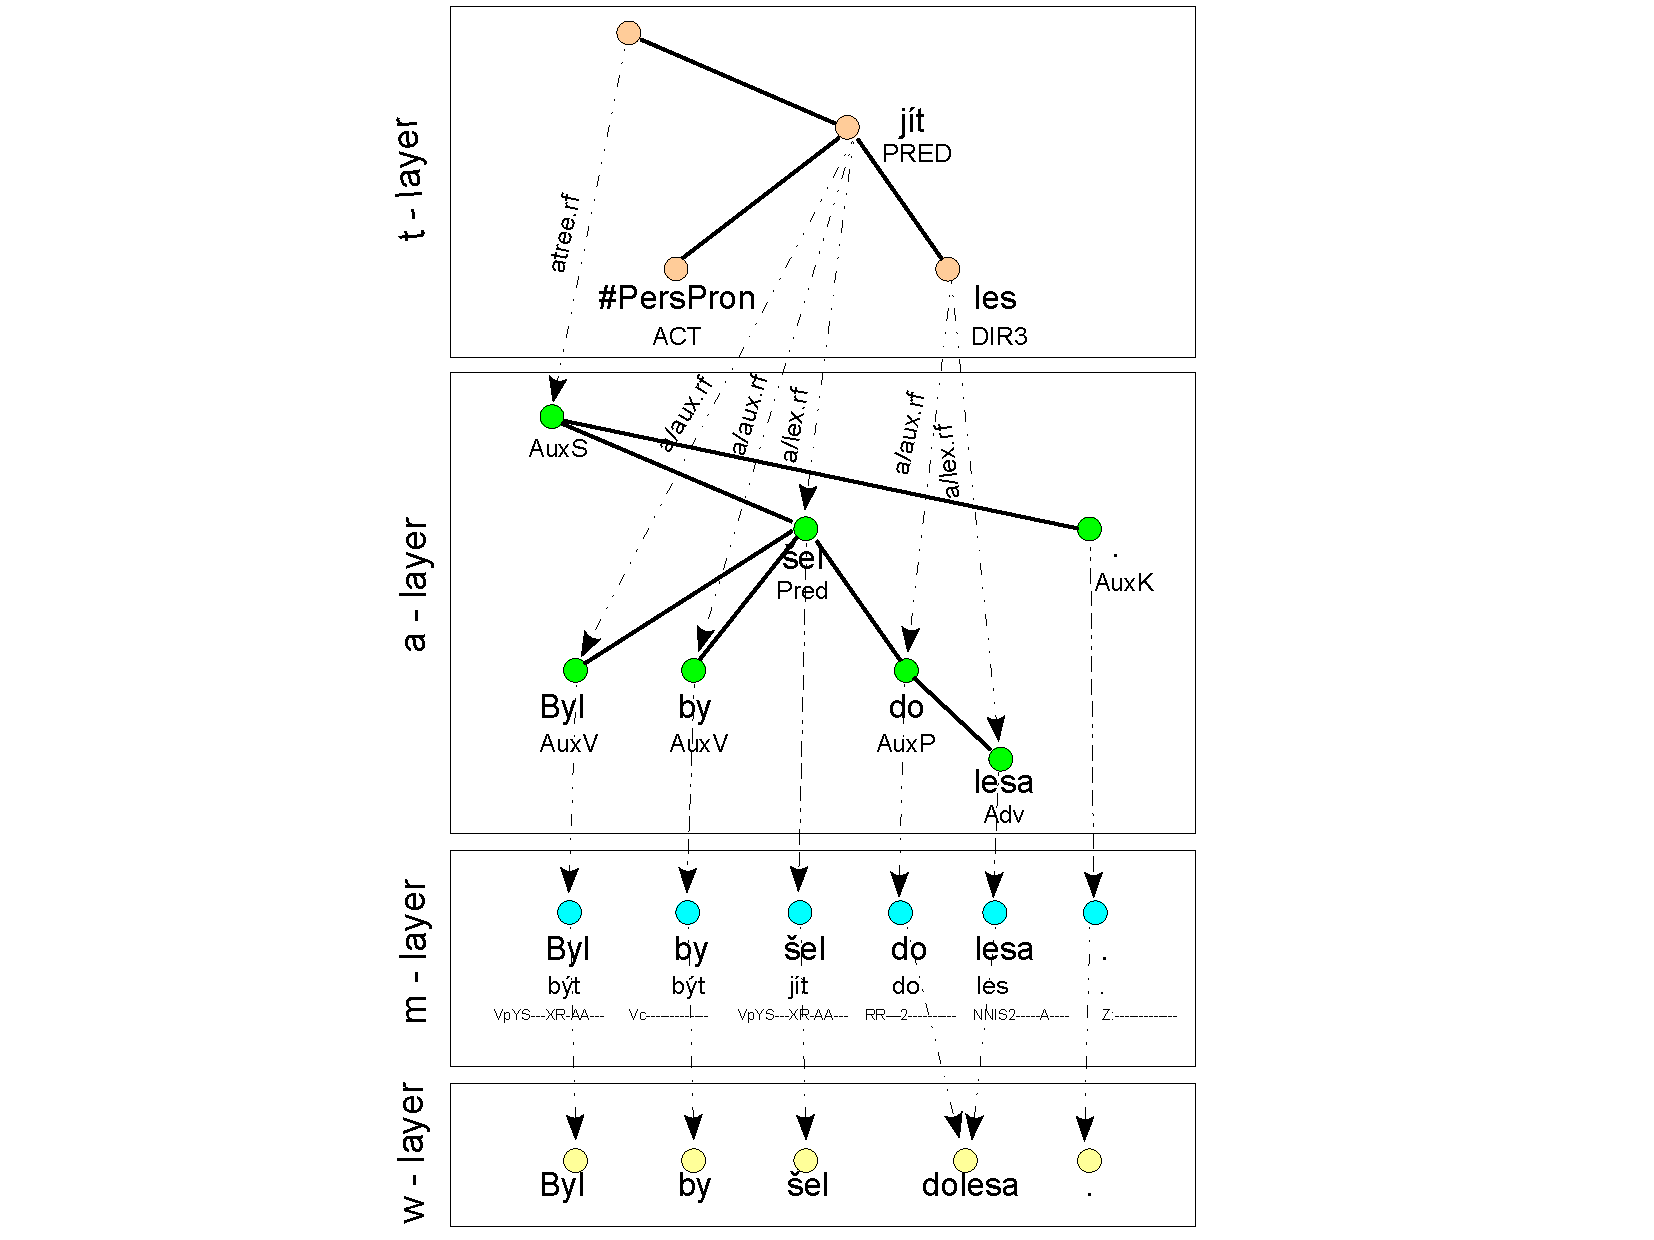
\includegraphics[scale=.38]{images/roviny.pdf} %180,0,580,595
%\begin{center}
%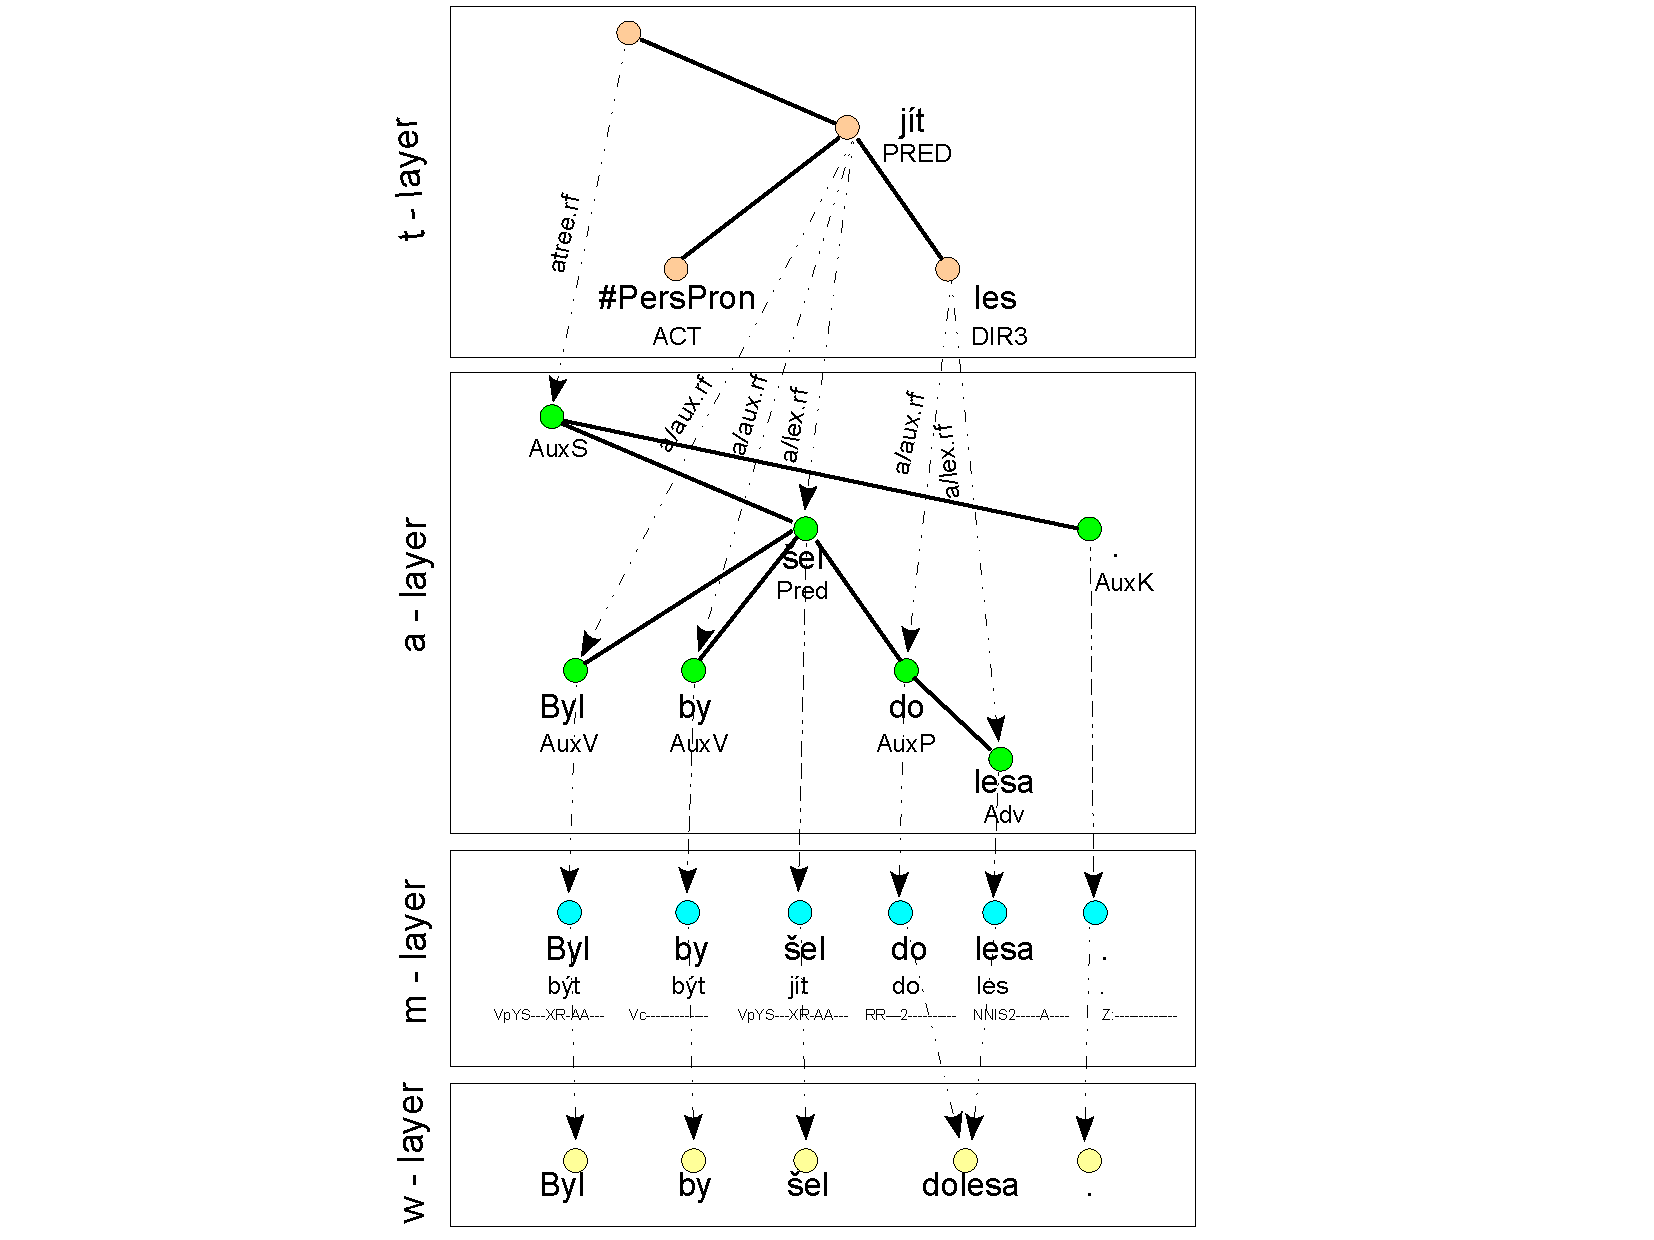
\epsfig{file=images/roviny.pdf,height=6cm,bbllx=100,bblly=425,bburx=300,
%        bbury=625,clip=}
%\end{center}
   \caption{The rendered Czech sentence \emph{Byl by šel dolesa}. (lit.: He-was would went toforest.) contains past conditional of the verb ``jít'' (to go) and a typo ``toforest'' repaired on m-layer.}
   \label{fig:layers}
\end{figure}

Our project aims at improving the current state of t-lemmas. Our goal is to assign each t-node a t-lemma that would correspond to a lexeme, i.e. that would really distinguish the t-node's lexical meanings. To achieve this goal, in the first phase of the project, which we report on in this paper, we \emph{identify multiword expressions and create a lexicon of the corresponding lexias}. A simple view of the result of our annotations is given in the Figure~\ref{fig:trees}, some technical details are in Section~\ref{sec:annot:analysis}.
%Remaining t-lemmas of ``single-word t-nodes'' will be examined and possibly changed later. But to do that, we must finish the current phase in order to know what the remaining ``single-word'' nodes are.

% to leave out ???
%There are also other quite practical motivations for MWE annotation: If we want to identify coreference relations between for instance ``Association for Computational Linguistics'', ``ACL'', and  ``it'' in a text, we need to identify the first expression as a single unit. For some applications we might also need to know what kind of entity it is. 

\begin{figure}[htbp]
   \centering
   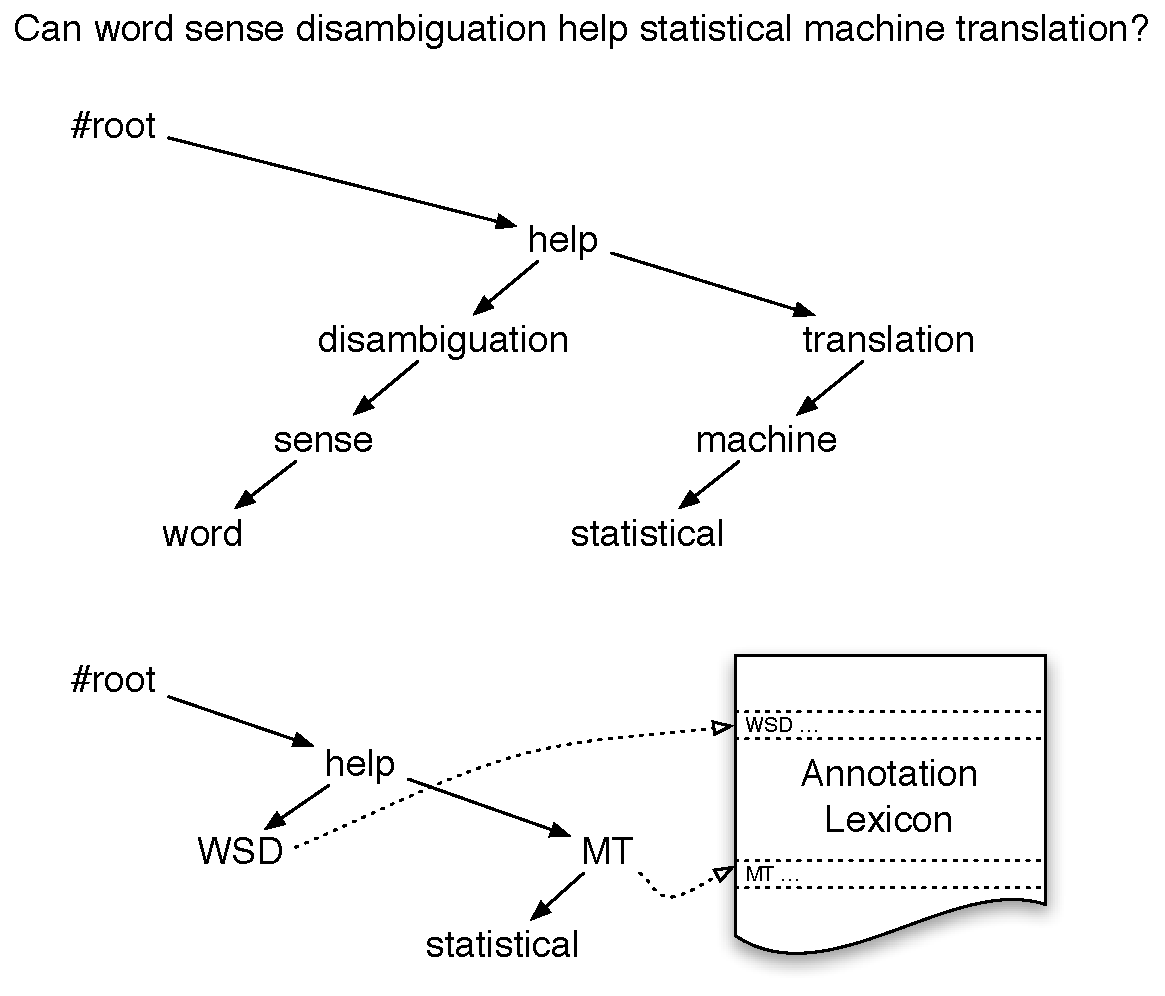
\includegraphics[width=3.4in]{images/stromecky.pdf}
   \caption{Schema of the changes in t-trees after integration of our annotations; every MWE forms a single node and has its lexicon entry}
   \label{fig:trees}
\end{figure}


In the Prague dependency treebank version 2.0 \citep{pdt2:2006} there are several functors that refer to multiword expressions (MWEs) in one way or another. There are also two technical lemmas \texttt{\#Idph} and \texttt{\#Forn} that identify roots of subtrees representing MWE's. Tectogrammatical annotation is described in detail in~\citet{mikulova:2006}.


\section{Search and visualisation tools}
\label{sec:pdt:tools}
There are currently three graphical search engines for PDT: Netgraph \citep{mirovsky:2009}, TrEd \citep{pajas:tred} and PML-TQ \citep{pmltq}. Both have their respective benefits, but since TrEd is considerably faster due to its use of an SQL database backend \citep{pmltq}, we have used TrEd for all the examples in this work. We also give the search queries using the PML Tree Query language designed by \citet{pmltq} where appropriate.

%%%%%%%%%%
\section{List structures}

\subsection{Foreign Phrase: \code{t-node [t\_lemma = \#Forn]}}\label{PDT:Forn}
Foreign Phrase seems to be overused and its overuse seems a bit arbitrary. \\
- jmena firem jsou nekdy forn, nekdy ne. (dohledat)\\

%%
\subsubsection{Foreign phrases with just one t-node}
There are 34 occurrences of this construction in the PDT~2.0. Counting them is as easy as writing a query in Figure~\ref{fig:tq-forn1} and extending it with this filter: \code{>>count(\$n)}.

\begin{wrapfigure}{r}{0.32 \textwidth}
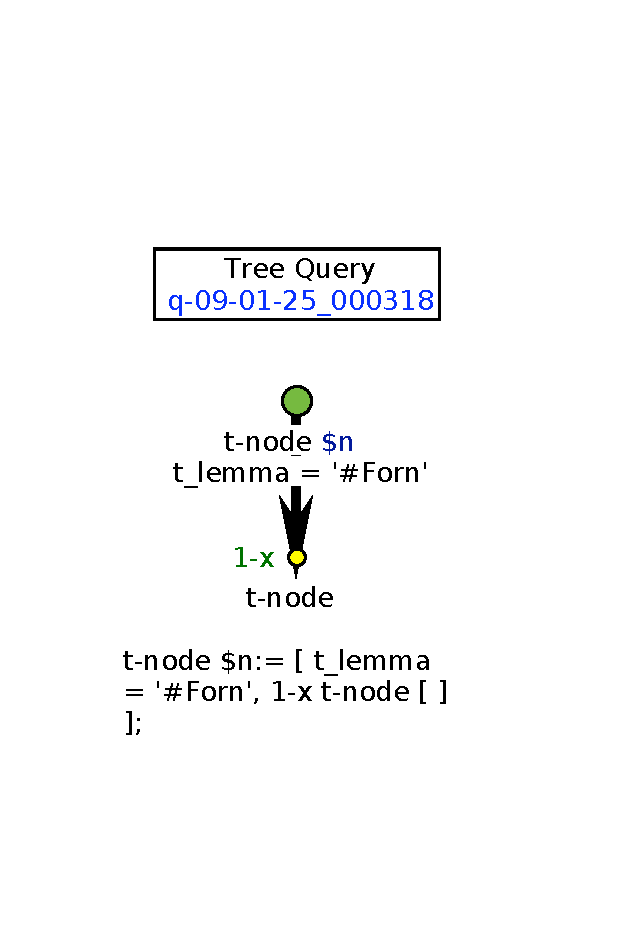
\includegraphics[width=0.3 \textwidth]{images/vyhledavky/query-forn-1-x.pdf}
\caption{PML-TQ search query for single-node foreing phrases}
\label{fig:tq-forn1}
\end{wrapfigure}

In case of the bibliographic reference in Figure~\ref{fig:forn-biblio} there is coordination of three foreign phrases corresponding to the parts of a bibliographic reference annotated, but the reason for this is not very clear. After all, the point of annotating foreign phrases as simple lists with a \code{\#Forn} node as a head was to make no assumptions about these pieces of a text \pageref{pdt-t-man:300}.  \\
- je to kvuli te interpunkci???

\begin{figure}[h]
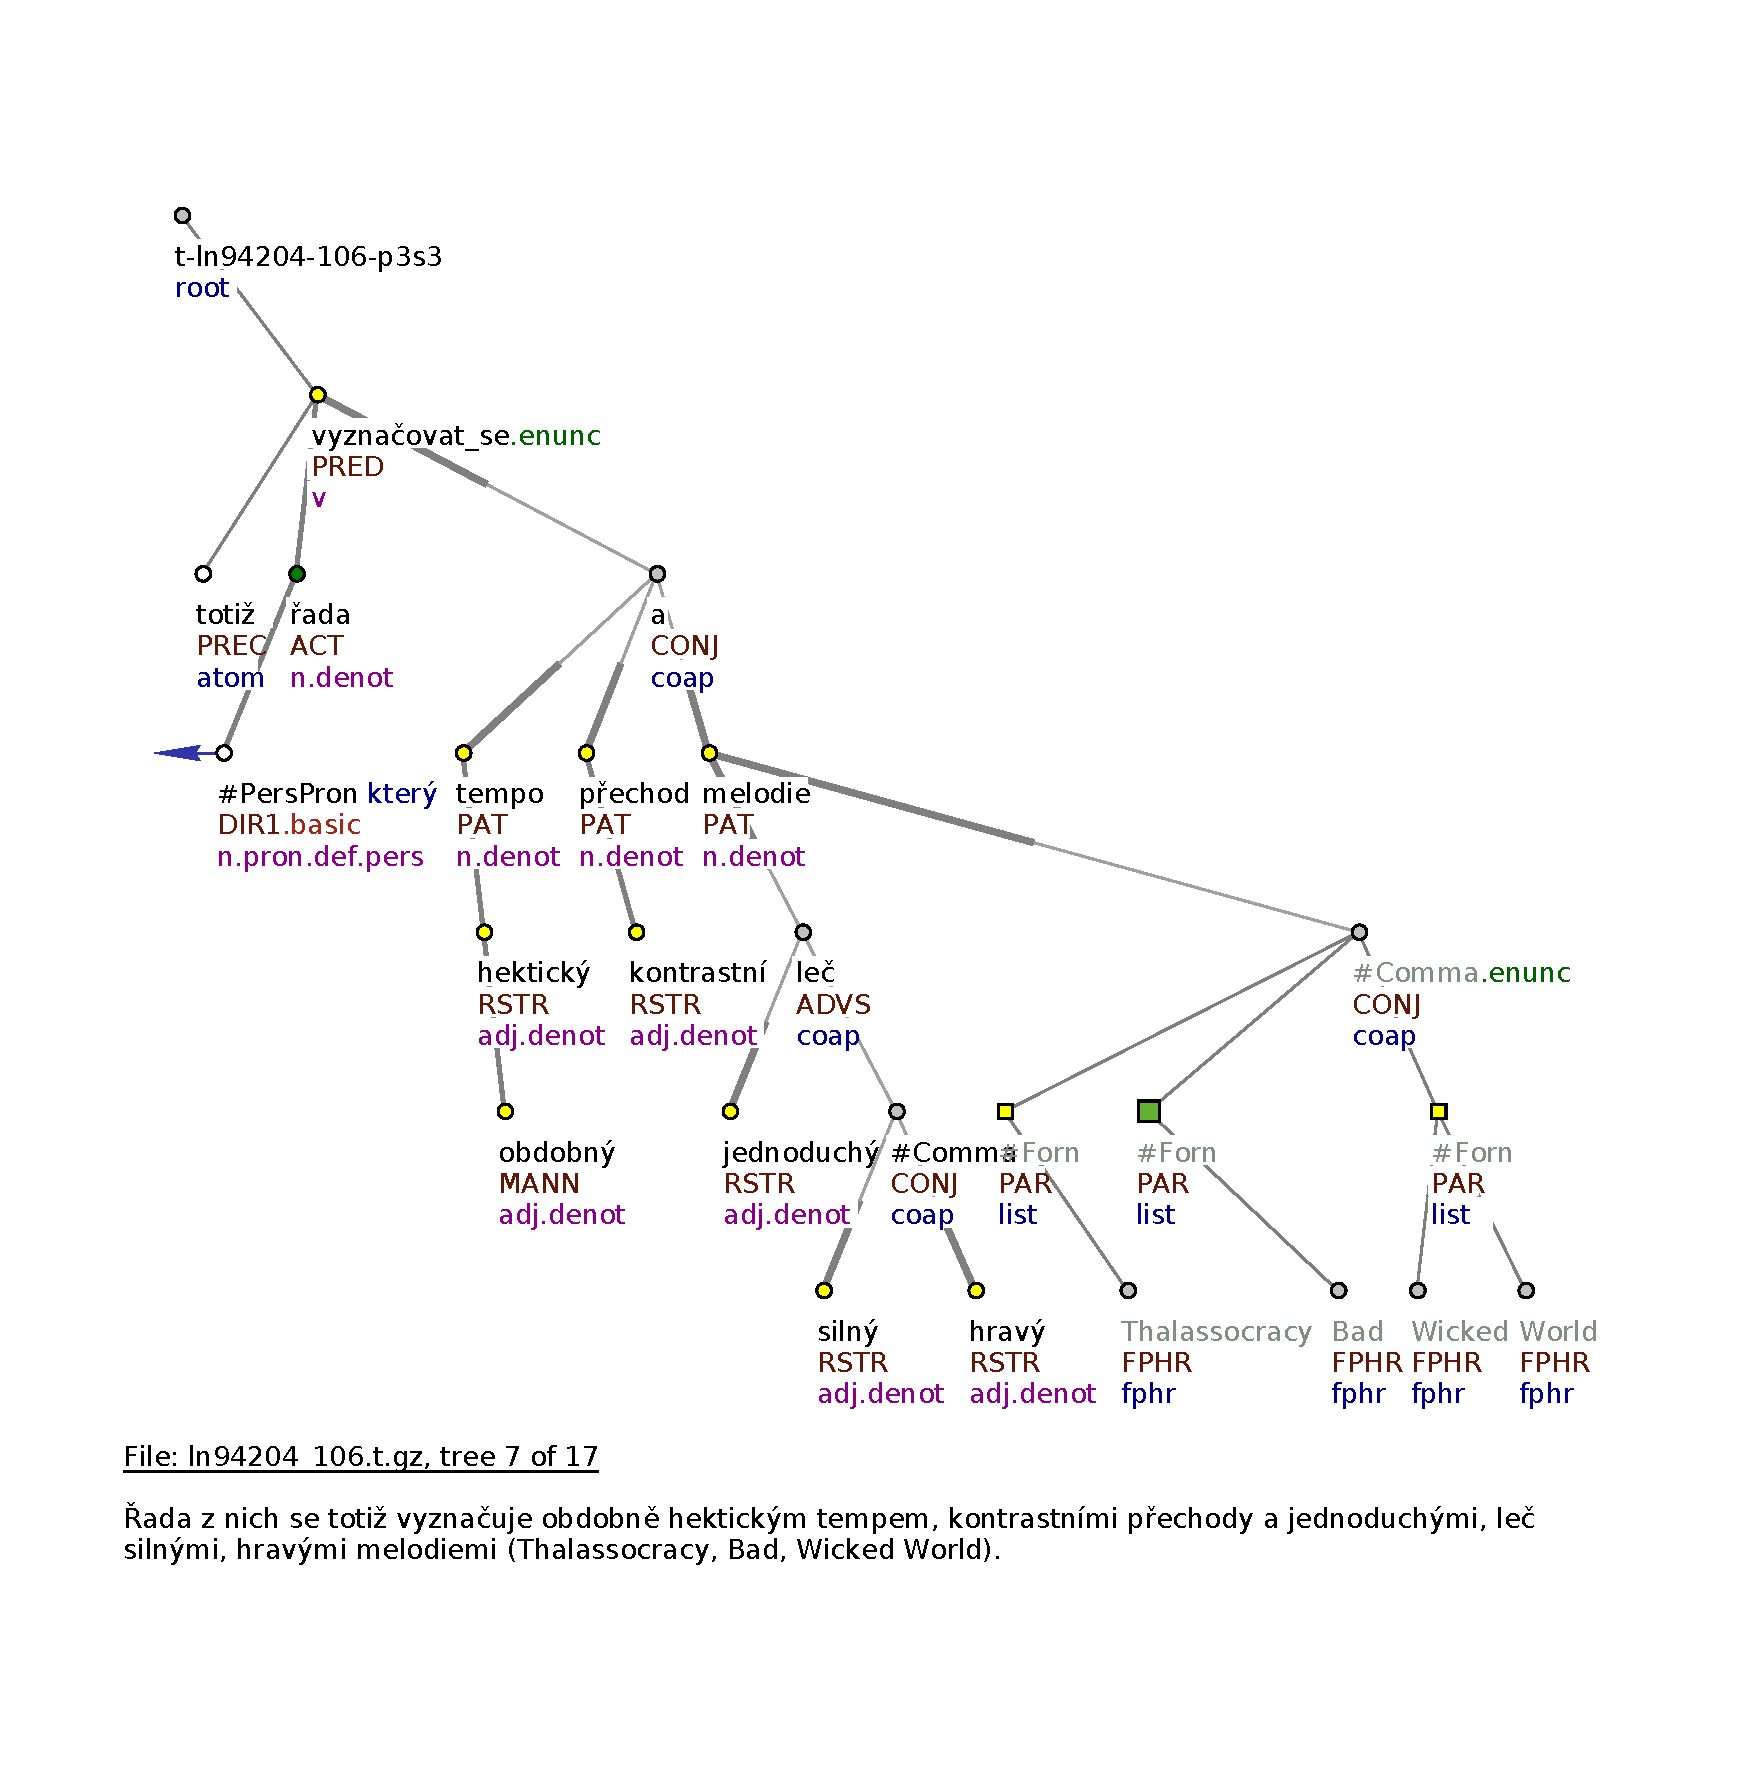
\includegraphics[width=\textwidth]{images/vyhledavky/forn-coord1x-biblio.pdf}
\caption{A bibliographic reference analysed as a coordination of three foreign phrases}
\label{fig:forn-biblio}
\end{figure}

Names of companies seem to be distinguished more by the country of origin then by any linguistic reasons, as demonstrated in Figure~\ref{fig:forn-firmy}. As far as linguistic criteria are concerned, Chemapol and Inekon are as foreign as Agip or Total. However the first two are, or at least were,%
\footnote{At the time of writing this thesis Chemapol is owned by another international company, which only emphasises vagueness of this distinction} %
%
Czech companies, while those in the latter group have a foreign origin.

\begin{figure}
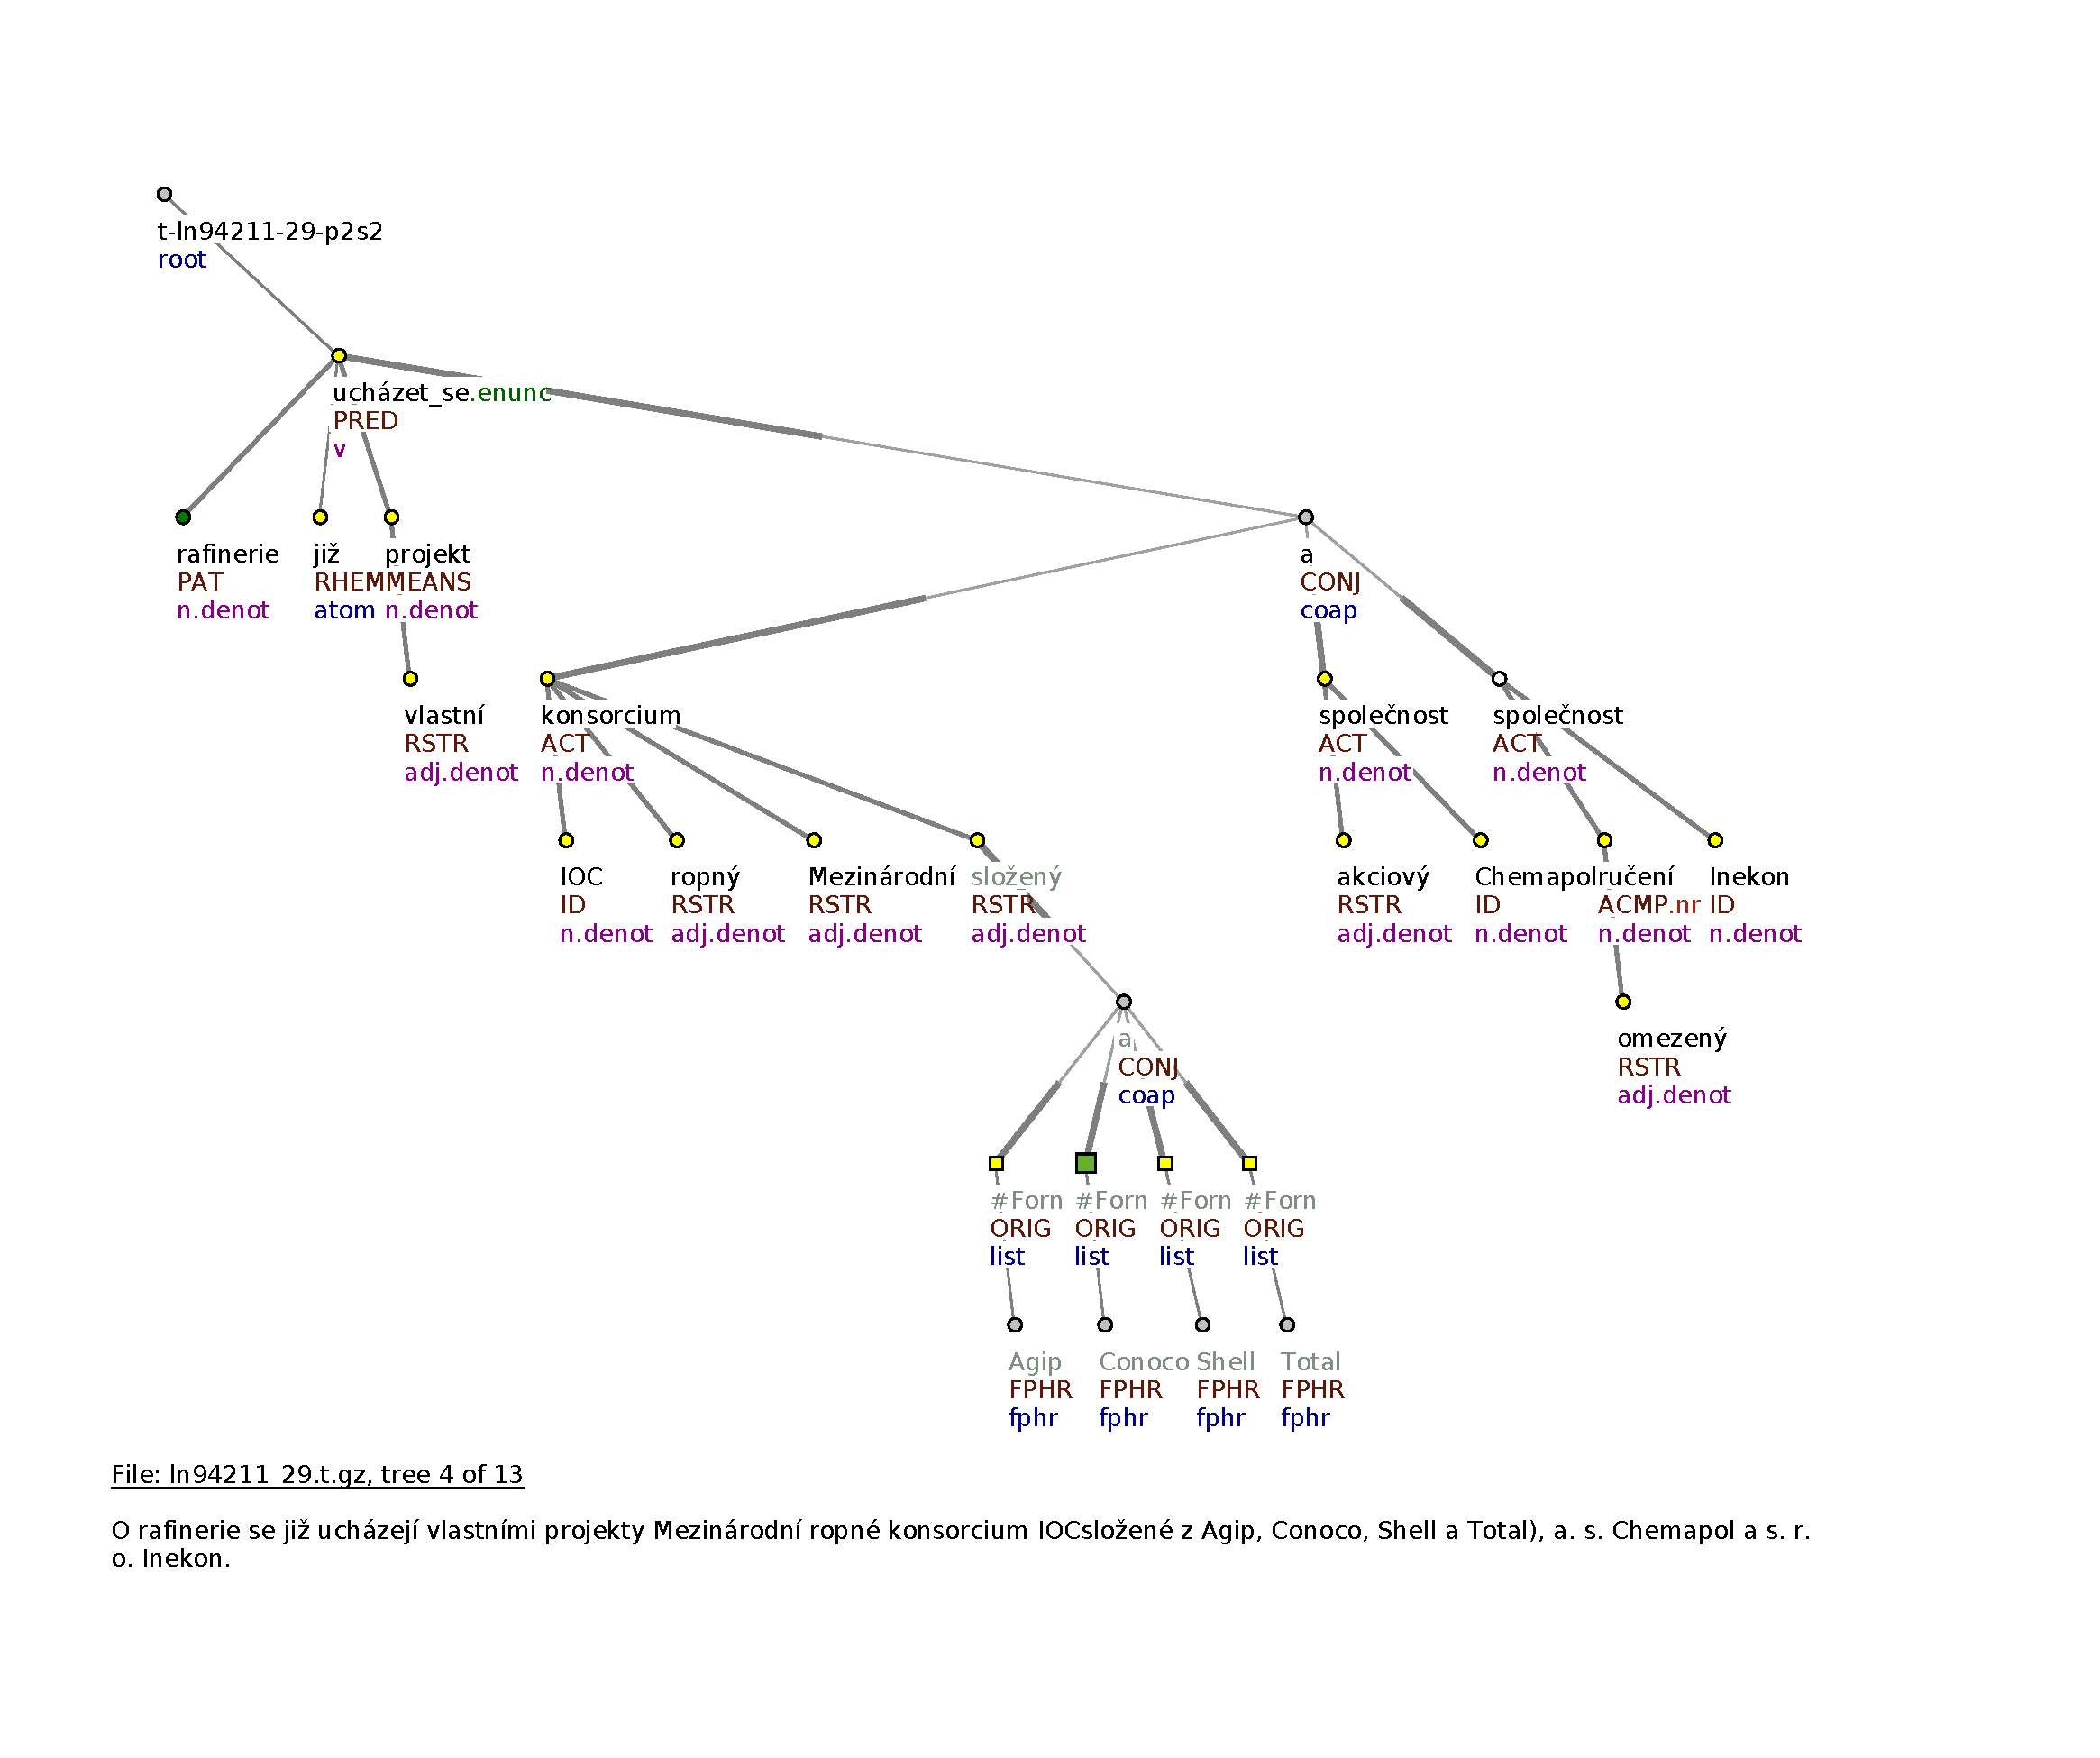
\includegraphics[width=\textwidth]{images/vyhledavky/nazvy-firem.pdf}
\caption{Annotation of Czech and foreign company names}
\label{fig:forn-firmy}
\end{figure}

%%%%%%%%%%
\section{CPHR and DPHR}

\subsection{CPHR}
There are 76 occurrences of {\tt CPHR} nodes, whose head verb is not its parent, but only effective parent, in 40 sentences. See Figure~\ref{fig:tq-echild} for the query and Figures~\ref{fig:cphr-echild} and~\ref{fig:cphr-echild2} for examples.
\begin{wrapfigure}{r}{0.32 \textwidth}
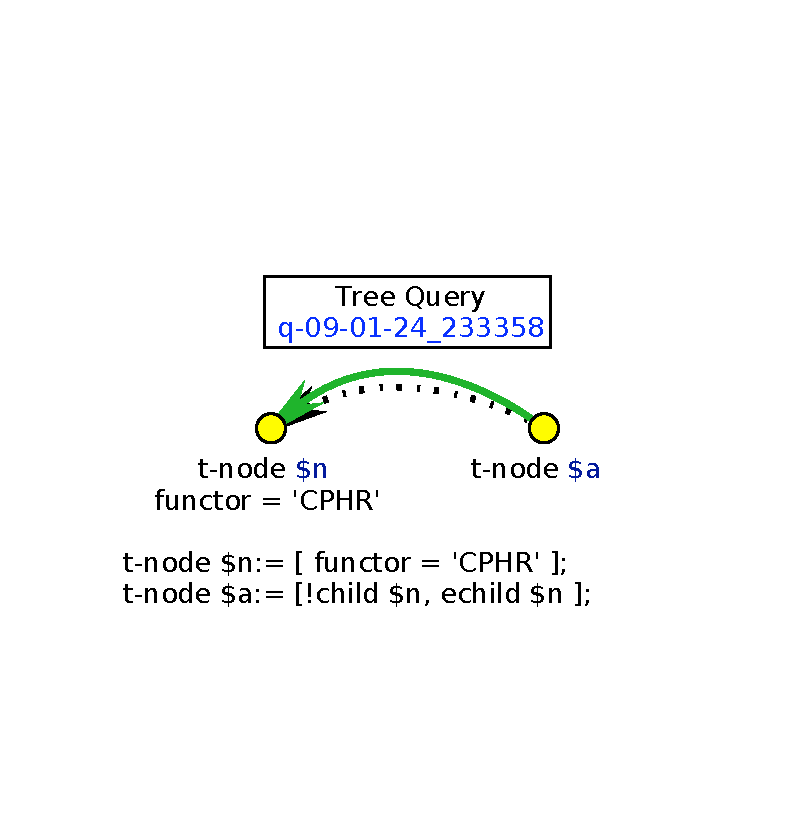
\includegraphics[width=0.3 \textwidth]{images/vyhledavky/query-echild.pdf}
\caption{PML-TQ search query for CPHR nodes, whose effective parrent is not its parent}
\label{fig:tq-echild}
\end{wrapfigure}

\begin{figure}[h]
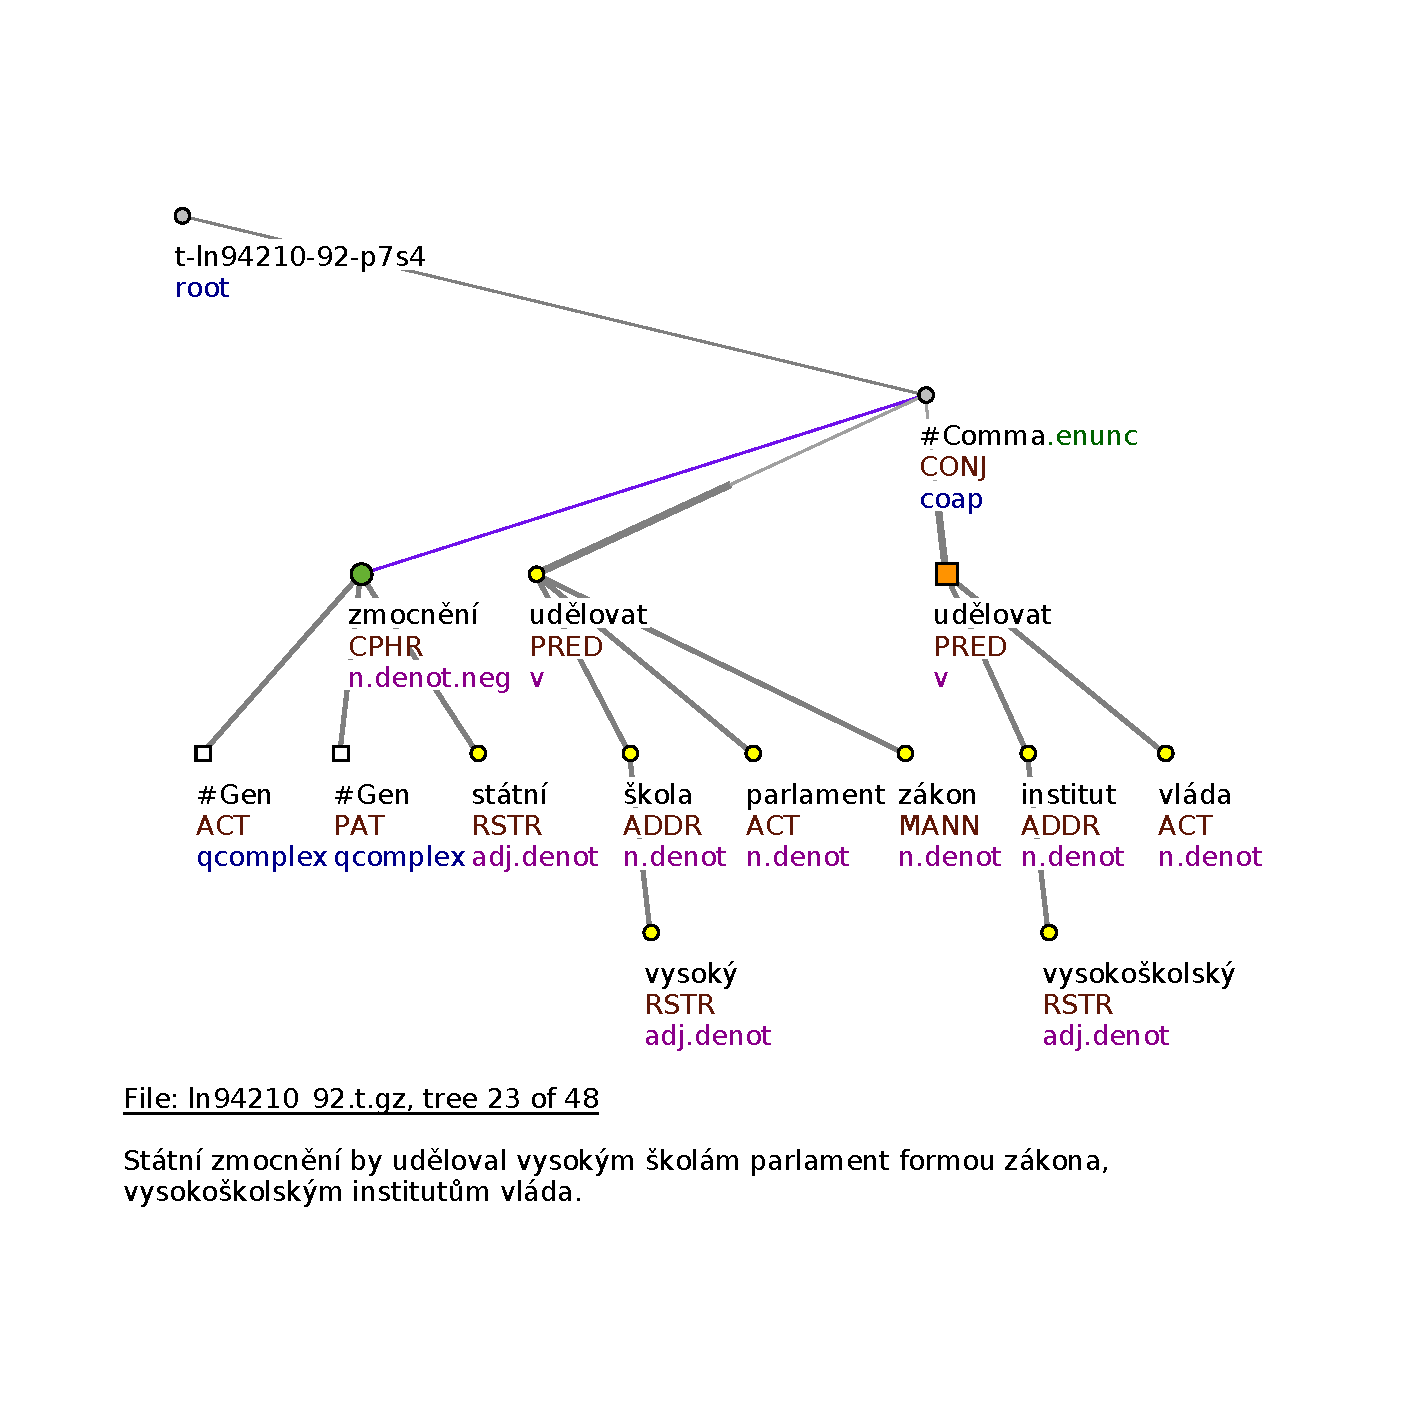
\includegraphics[width=0.8\textwidth]{images/vyhledavky/cphr-echild.pdf}
\caption{Coordination of verbonominal idioms, where the verbal parts are further ???rozvite }
\label{fig:cphr-echild}
\end{figure}

Figure~\ref{fig:cphr-echild2} shows on the other hand a coordination of two V-N idioms with the same verbal part.
\begin{figure}[h]
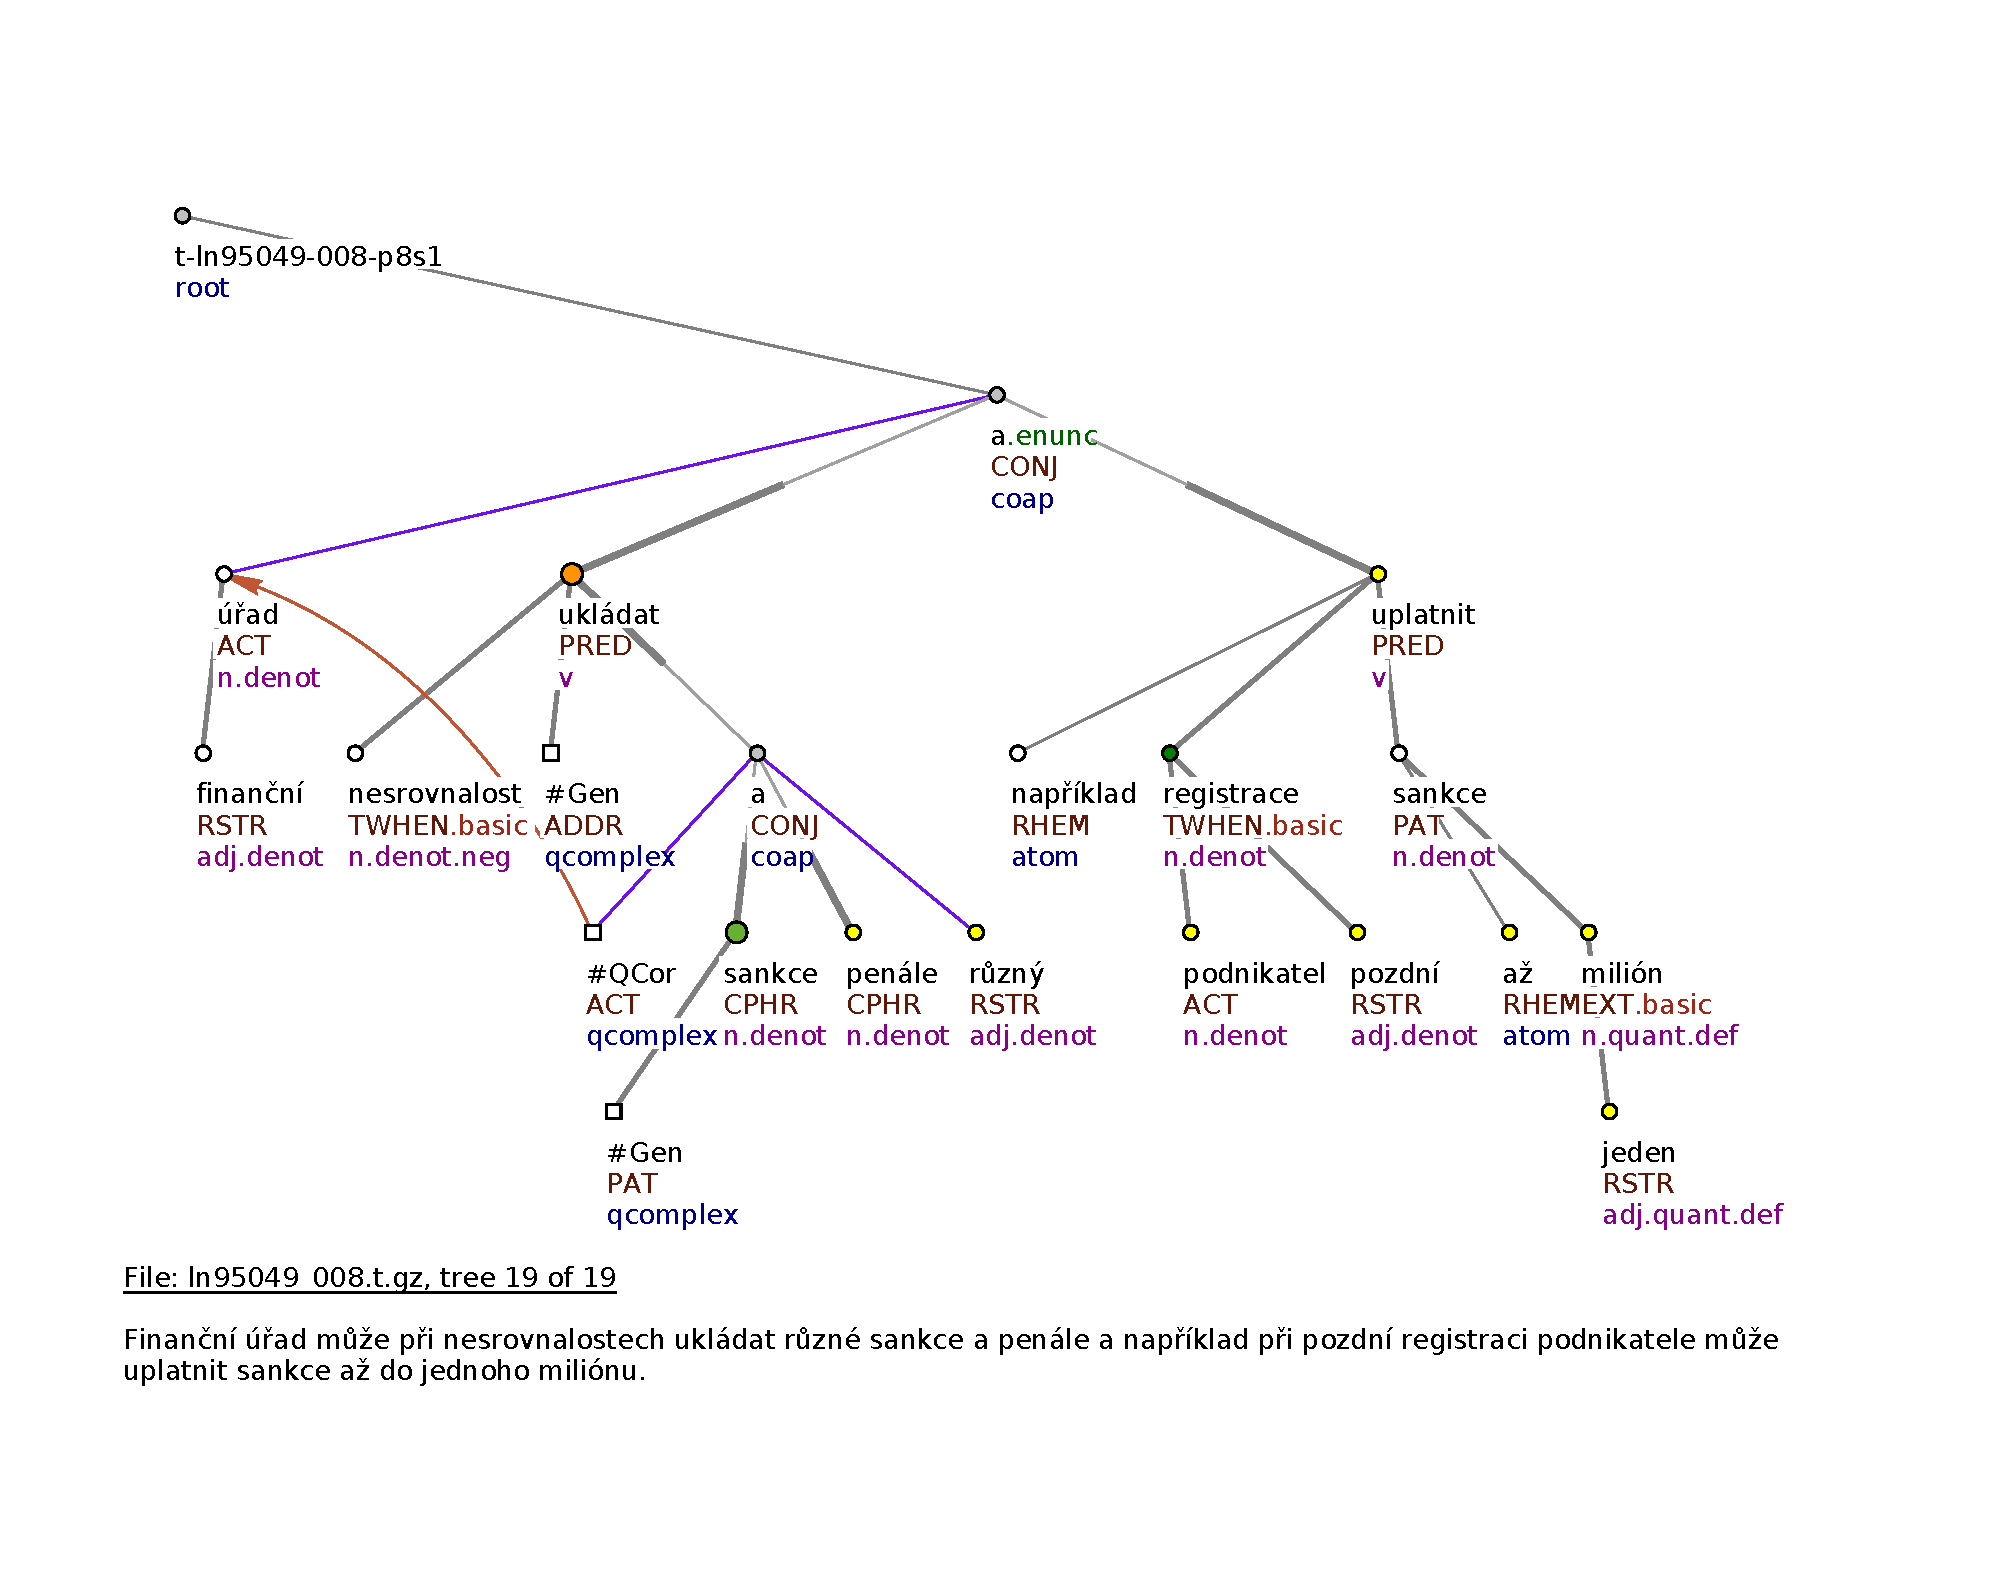
\includegraphics[width=\textwidth]{images/vyhledavky/cphr-ukladat-sankce-a-penale.pdf}
\caption{Coordination of two idioms starting with the same verb}
\label{fig:cphr-echild2}
\end{figure}


%%%%%
\section{JLRE -- Current state of MWEs in PDT 2.0}
\label{sec:pdt:mwes}

During the annotation of valency, which is a part of the tectogrammatical layer of PDT 2.0, the t-lemmas, have been basically identified for all the verbs and some nouns and adjectives.
The resulting valency lexicon is called PDT-VALLEX \citep{hajic:2003} and we can see it as a repository of lexemes based on verbs, adjectives and nouns in PDT that have valency.
%
\footnote{It is so because in PDT-VALLEX valency is not the only criterion for distinguishing frames (=meanings). Two words with the same morphological lemma and valency frame are assigned two different frames if their meaning differs.} 

This is a starting point for having t-nodes corresponding to lexemes. However in the current state it is not fully sufficient even for verbs, mainly because parts of MWEs are not joined into one node. Parts of frames marked as idiomatic are still represented by separate t-nodes in a tectogrammatical tree (e.g.~nodes with t-lemmas {\tt“co”} in Figure~\ref{fig:co-nevidet} or {\tt“k\_dispozici”} in Figure~\ref{fig:asistent}). Verbonominal phrasemes are also split into two nodes, where the nominal part is governed by the verb. Non-verbal idioms have not been annotated at all in the current state of PDT. 

In Figures~\ref{fig:co-nevidet}, \ref{fig:klaus}, and \ref{fig:asistent} we give several examples of t-trees in PDT 2.0, that include idioms, light verb constructions and named entities:
\begin{figure}[htbp]
   \centerline{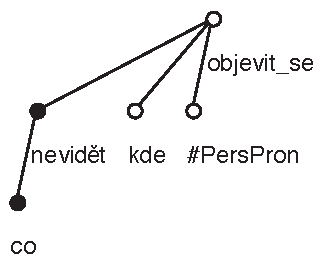
\includegraphics[scale=.7]{images/co-nevidet-clause.pdf}}
   \caption{\label{fig:co-nevidet}Idiom \emph{Co nevidět} meaning ``in a blink (of an eye)'', (literally: what not-see)}
\end{figure}

\begin{figure}[htbp]
   \centerline{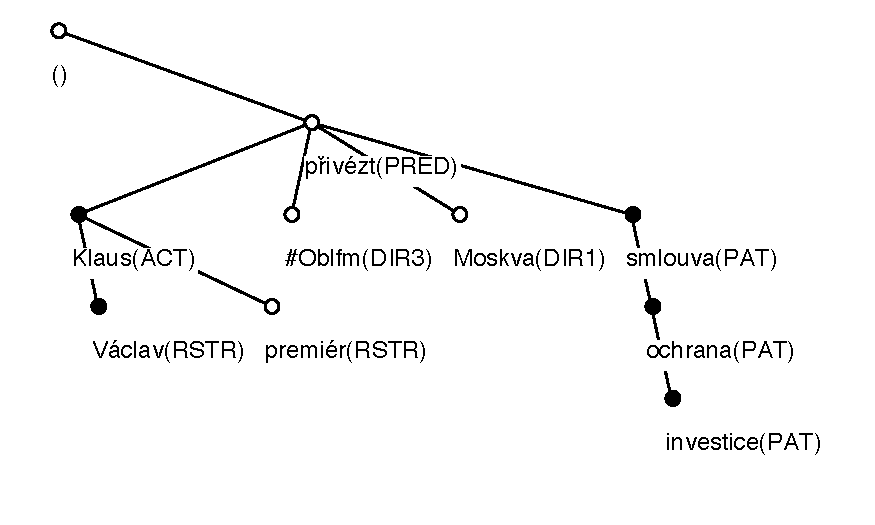
\includegraphics[width=3.7in]{images/klaus-a-smlouva.pdf}}
   \caption{A sentence featuring a personal name and a name of a bilateral treaty (which is not the exact official name, however, thus it is not capitalised)}
   \label{fig:klaus}
\end{figure}

\begin{figure}[htbp]
   \centerline{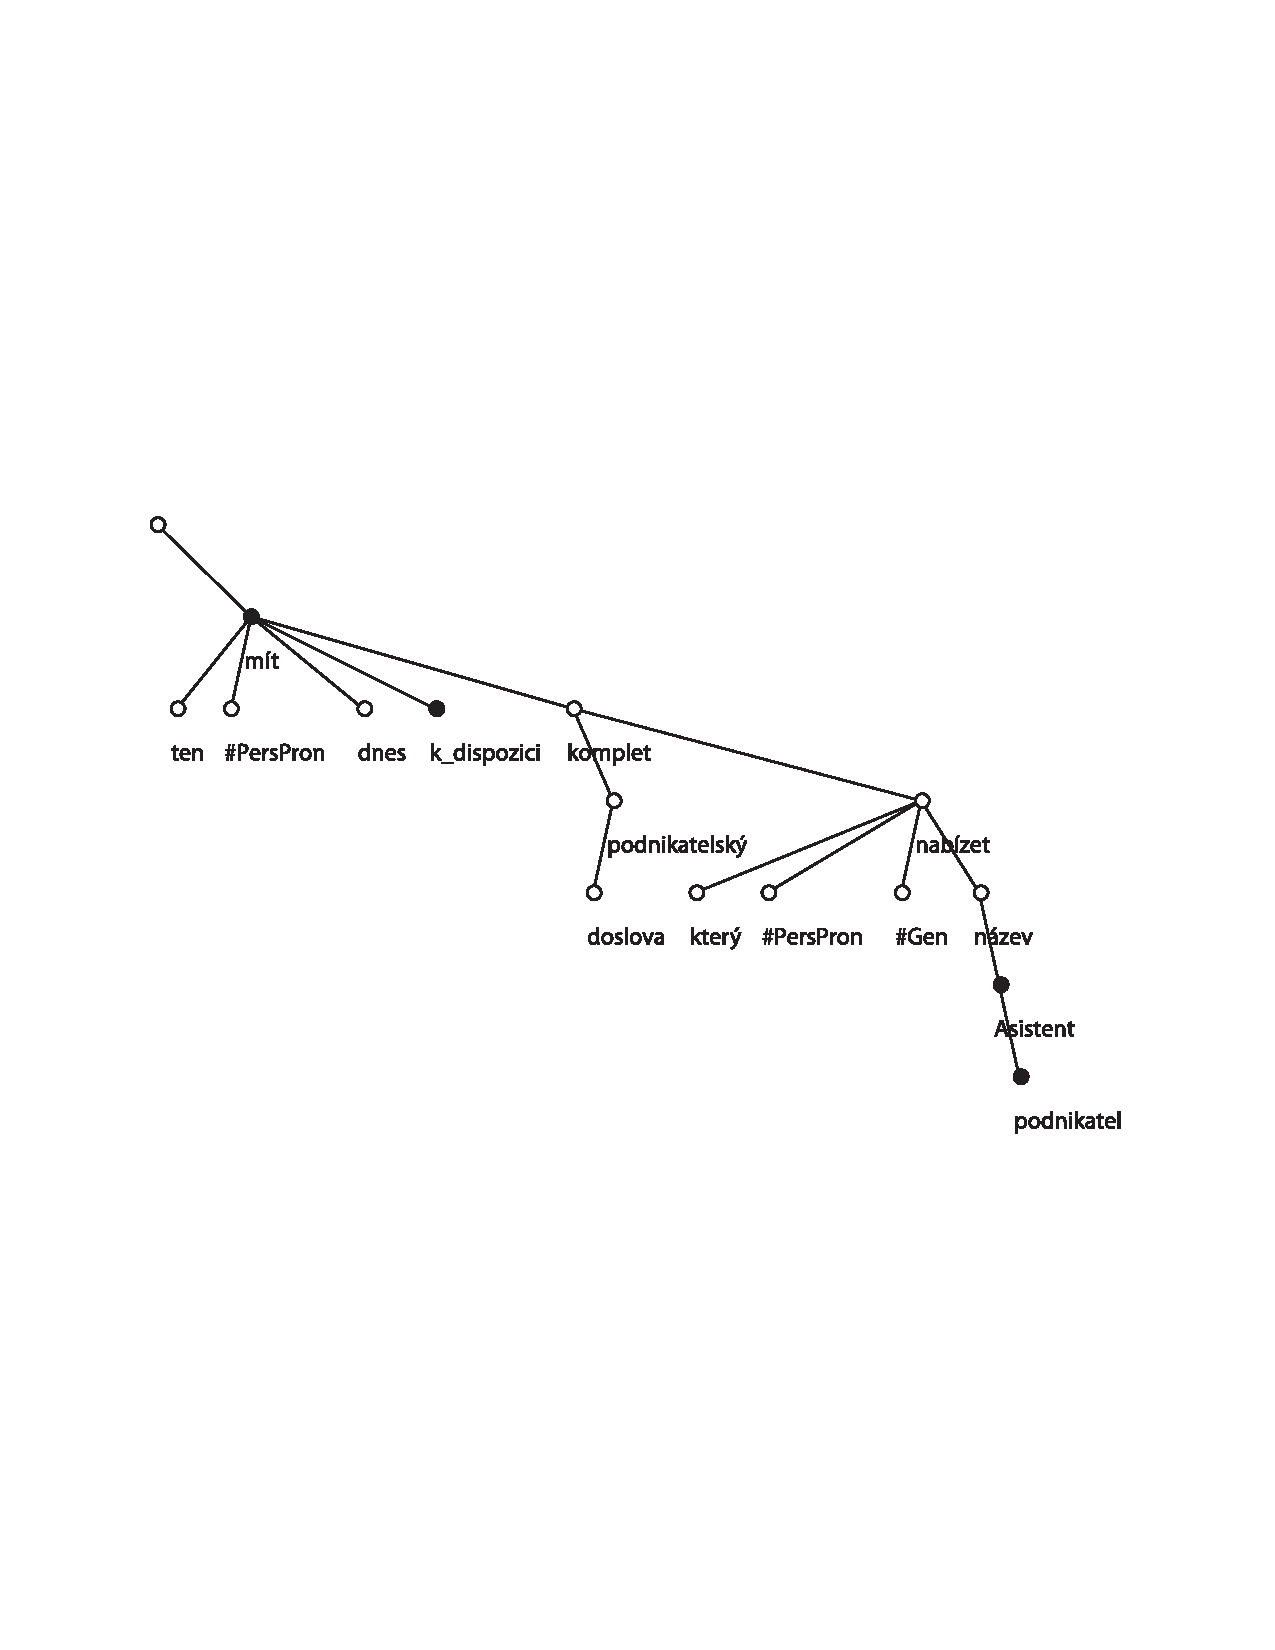
\includegraphics[height=2.6in]{images/as-pod.pdf}}
   \caption{A t-tree of a sentence featuring a light verb construction \emph{mít k dispozici} (lit.: to have at [one's] disposal) and a named entity (a product name\emph{Asistent podnikatele} (lit.: assistant of-businessman) that looks like a common phrase, except for the capital `A'.}
   \label{fig:asistent}
\end{figure}

%[[!!! doplnit informaci o seznamových strukturách s kořenem \#Idph či \#Forn.]]

% !TEX root = ../disertace.tex
%!TEX encoding = UTF-8 Unicode

\chapter{Annotation}
\label{sec:annot}

\section{Annotation – JLRE -- prekryv s kapitolou s-data a \seman}
\label{sec:annot:jlre}

PDT 2.0 uses PML~\citep{pajas:2005}, which is an application of XML that utilizes a stand-off annotation scheme. We have extended the PDT-PML with a new schema for so-called s-files. We use these files to store all of our annotation without altering the PDT itself.
These s-files are very simple: basically each of them corresponds to one file of PDT and consists of a list of s-nodes. Each s-node corresponds to an occurrence of a MWE and is composed of a link to an entry in SemLex and a list of identifiers of t-nodes that correspond to this \mbox{s-node}. Figure~\ref{fig:s-layer} shows a relation of s-layer to PDT layers and SemLex.\footnote{Although we have created the PML schema of s-layer primarily for annotations of MWEs, we made it quite generic. It can be utilized for any treebank annotations that use a large lexicon. For instance one s-file can contain multiple annotations of valency referencing to different valency dictionaries. This generic nature of s-layer is the reason why it allows references to morphological, analytical or tectogrammatical layer of PDT, even though in our current project we only need the references to t-layer.}
%\colorbox{yellow}{TODO: odkaz na užití v anotacích podle CWN.}}.
\begin{figure}[htbp]
   \centering
   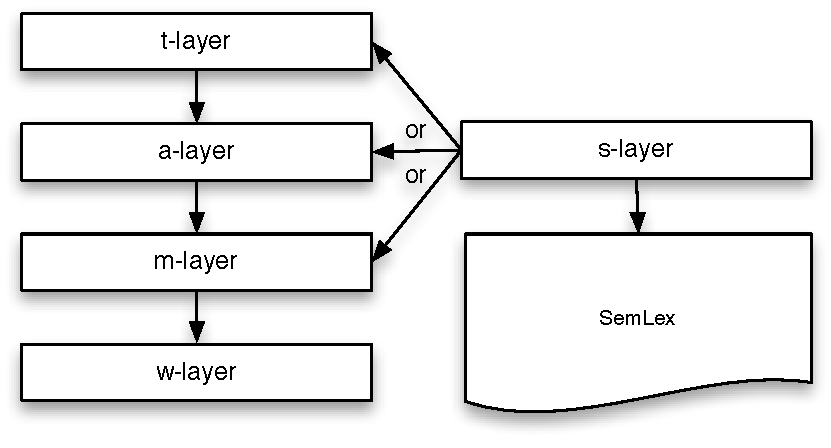
\includegraphics[scale=.5]{images/layers-with-s-layer.pdf} % requires the graphicx package
   \caption{Relation of s-layer to PDT and SemLex}
    \label{fig:s-layer}
\end{figure}


Our annotation program reads in a tectogrammatical representation (t-file) and calls TrEd \citep{pajas:tred} to generate plain text. This plain text (still linked to the tectogrammatical representation) is presented to the annotator. While the annotator marks MWEs already present in SemLex or adds new MWEs into SemLex, tree representations of these MWEs extracted from underlying t-trees are added into their SemLex entries via TrEd scripts. 

%These tree representations are quite simple: for each node in a MWE we only record its t-lemma and its father's ID.


%%%%%
\section{Pre-annotation}
\label{sec:annot:pre}
Because MWEs tend to occur repeatedly in a text, we have decided to test pre-annotation both for speed improvement and for improving the consistency of annotations. 
%We work o
On the assumption that \emph{all occurrences of a MWE share the same tree structure}, while there are no restrictions on the surface word order other than those imposed by the tree structure itself
%
% pre-annotation types
%W
we have decided to employ four types of pre-annotation:

\begin{asparaenum}[A)]
\item \label{pre-hnatkova}External pre-annotation provided by Milena Hnátková (see~\citealp{hnatkova:2002}). With each MWE a set of rules is associated that limits possible forms and surface word order of parts of a MWE. This approach was devised for corpora that are not syntactically annotated and is very time consuming.
\item \label{pre-static}Our one-time pre-annotation with those MWEs from SemLex that have been previously used in annotation, and thus have a tree structure as a part of their entry.
\item \label{pre-on-load}Dynamic pre-annotation as in \ref{pre-static}, only with the SemLex entries that have been recently added by the annotator. 
\item \label{pre-on-annot}When an annotator tags an occurrence of a MWE in the text, other occurrences of this MWE in the article are identified automatically.%
%
\footnote{This is exactly what happens:
\begin{inparaenum}[1)]
\item Tree structure of the selected MWE is identified via TrEd
\item The tree structure is added to the lexeme's entry in SemLex
\item All the sentences in the given file are searched for the same MWE using its tree structure (via TrEd)
\item Other occurrences returned by TrEd are tagged with this MWE's ID, but these occurrences receive an attribute ``auto'', which identifies them (both in the s-files and visually in the annotation tool) as annotated automatically.
\end{inparaenum}
} % end footonote
\end{asparaenum}

Pre-annotation (\ref{pre-hnatkova})~was executed once for all of the PDT. (\ref{pre-static})~is performed each time we merge MWEs added by annotators into the main SemLex. We carry out this annotation in one batch for all PDT files remaining to annotate. (\ref{pre-on-load})~is done for each file while it is being opened in the annotation environment. 
(\ref{pre-on-annot})~happens each time the annotator adds a new MWE into SemLex and uses it to annotate an occurrence in the text. In subsequent files instances of this MWE are already annotated in step (\ref{pre-on-load}), and later even in (\ref{pre-static}).
%, when the lexia (lexicon entry) is merged into the main SemLex. 
 
\xxx{PRO FUTURA
We have currently performed double blind annotation of a part of data without pre-annotation (\ref{pre-static}) and (\ref{pre-on-load}). We also have smaller samples annotated without any pre-annotation and only with pre-annotation (\ref{pre-hnatkova}). Analysis of this data is necessary  to show that our assumption is correct and all the occurrences of a lexia share the same tree structure. Then we can safely add remaining pre-annotation steps. Provided the inter-annotator agreement is good enough we can also stop our current (rather expensive and time consuming) practice of double annotation of each file and comparing the annotations.} % end XXX

After the pilot annotation without pre-annotation (\ref{pre-on-annot})  we have compared instances of the same tags and found that 10.5\% of repeated MWEs happened to have two different tree representations. Below we analyse several most important sources of these inconsistent t-trees and possible improvements:
\begin{itemize}
%
\item \emph{Occasional lemmatisation errors.} They are not very frequent, but there is no efficient way to find and correct them before the annotations. So there is not much we can do but it is not very important. Our annotations can however serve as a source for automatic corrections.
	\begin{itemize}
	\item \textit{jižní Korea {\rm vs.} Jižní Korea} (southern vs. South Korea)
	\end{itemize}
% chyba anotatora (neoznaci v LexSemAnnu slovo)
\item \emph{Annotator's mistake (not marking correct words).} When an annotator makes an error while marking a first occurrence of a MWE, the tree representation that gets stored in SemLex is incorrect. As a result, pre-annotation gives false positives or fails to work. 

It is therefore necessary to allow annotators to correct the tree structure of a SemLex entry, i.e. extend functionality of the annotation tool. Once all the types of pre-annotation are employed, this error can happen only once, because all the following occurrences of a MWE are pre-annotated automatically. We are currently working on these improvements.
%
\item \emph{Gender opposites, diminutives and augmentatives.} These are currently represented by variations of t-lemma. 
We believe that they should be represented by attributes of t-nodes %, which would explicate information that is now given only implicitly. 
that could be roughly equivalent to some of the lexical functions in the Meaning-text theory (see \cite{melcuk:1992}).
This should be tackled in some future version of PDT. Once resolved it would allow us to identify following (and many similar) cases automatically. 
	\begin{itemize}
	\item \textit{obchodní ředitel {\rm vs.} obchodní ředitelka} \\(lit.: managing director-man vs. m. director-woman)
	\item \textit{rodinný dům {\rm vs.} rodinný domek} \\(lit.: family house vs. family little-house; but the diminutive \emph{domek} means basically “family house”)
	\end{itemize}
%
Currently we annotate these cases with the same MWE, but all the instances with the derived variants of t-lemma (like \emph{ředitelka } or \emph{domek} must be identified manually (see Section~\ref{sec:pre}). We plan to try automatic identification of some diminutives and gender opposites derived by most common patterns.

%
\item \emph{Newly established t-nodes corresponding to elided parts of MWEs in coordinations.} Since t-layer contains many newly established t-nodes, many of which cannot be lexicalised, our original decision was to hide all of these nodes from annotators and generate for them pure surface sentence. This decision resulted however in the current situation, when some MWEs in coordinations cannot be correctly annotated. 
%It is necessary to elide common part of coordinated multiword lexeme. 
For instance \emph{První a druhá světová válka} (First and Second World War) is a coordination of two multiword lexemes. A tectogrammatical tree that includes it does have newly established t-nodes for “world” and “war” of the first lexeme but they are elided in the surface sentence. 

After analysing annotated examples like the one above we have decided to generate surface words from some of the newly established t-nodes in order to allow correct annotation of all the MWEs. These ``added'' words will be displayed in grey and while some morphological forms of these words may be incorrect, we believe they will serve their purpose.

{\xxx The first lexeme cannot be identified automatically. In this and other similar cases t-nodes for elided parts of multiword lexemes should have been part of PDT, in our opinion. Given that our goal is to have one t-node for each lexia, however, we believe it would not be efficient to invest substantial amount of manual work into adding these elided t-nodes now only to eliminate them more efficiently in near future. We can just as well leave it to our annotators to identify these instances of MWEs (it is as common for NEs, as it is for lexias) manually.

\item \emph{Bridging anaphora} e.g. Ceska narodni banka <- banka \\
Since in the context the second expression stands for the first only with some words ellided, our annotators were instructed to annotate it as an instance of the lexia \emph{Česká národní banka}. 
This problem could be solved by annotations of coreference. If the coreference between nominal expressions was present in the PDT 2.0, our annotators would simply mark the first occurence and all the anaphoric expressions would be marked automatically. 
} % end xxx
\end{itemize}


\xxx{
\emph{spojit s 'itemize' vyse!}\\
because these cases are caused by ellipses, variations in lexical form such as diminutives etc., or wrong lemmatisation, rather than inconsistencies in the tree structure. These cases show us some problematic issues in PDT 2.0, for instance:
\begin{itemize}
\item \textit{jižní Korea {\rm vs.} Jižní Korea} \\(southern vs. South Korea) -- wrong lemmatisation
\item \textit{obchodní ředitel {\rm vs.} obchodní ředitelka} \\(lit. managing director-man vs. m. director-woman) -- in future these should have one t-lemma. Morphological gender should be specified by an attribute of a t-node.
\end{itemize}
} % end xxx


Up to now we have not found any MWE such that its structure cannot be represented by a single tectogrammatical tree. 1.1\% of all occurrences were not connected graphs, but this happened due to errors in data and to our incorrect handling of coordinations with newly established t-nodes (see above). This corroborates our assumption that (disregarding errors) all occurrences of a MWE share the same tree structure. As a result, we started storing the tree structures in the SemLex entries and employ them in pre-annotation (\ref{pre-on-annot}). This also allows us to use pre-annotations (\ref{pre-static}) and (\ref{pre-on-load}), but we have decided not to use them at the moment, in order to be able to evaluate each pre-annotation step separately. Thus the following section reports on the experiments that employ pre-annotations (\ref{pre-hnatkova}) and (\ref{pre-on-annot}).


%%%%%
\section{Analysis of interannotator agreement – JLRE}
\label{sec:annot:analysis}
Two annotators have started to use (and test) the tool we have developed.
They both have got the same texts. The text is generated from the t-trees and presented as a plain text with pre-annotated words mark\-ed by colour labels. Annotators add their tags in the form of different colour labels and they can delete the pre-annotated tags. 
In this experiment the data consists of approx. 310,000 tokens, which correspond to 250,000 t-nodes.
Both annotators have marked about 37,000 t-nodes ($\approx$ 15\%) as parts of MWEs and grouped them into 17,000 MWEs. So the average length of a MWE is 2.2 t-nodes.
% Annotator $A$ %Vimmrova
% has grouped them into 7,263 MWEs and annotator $B$ %Sidak
% into 6,888. So the average length of a MWE is 2.2 t-nodes.

The ratio of general named entities versus SemLex entries was 50:50 for annotator $A$ and 52:48 in the case of annotator $B$. Annotator $A$ used SemLex more frequently (than she used named entities and also than annotator $B$ used SemLex), but did not utilise as many lexicon items as annotator $B$.
% Annotator $B$ used 10\% more lexias than annotator $A$ (3,279 and 3,677), while they both used almost the same number of NEs.
This and some other comparison is given in Table~\ref{tab:anot}.


\begin{table}[h]
\centering
\begin{tabular}{l|r|r}
type of MWE&$A$&$B$\\
\cline{1-3}
SemLex entries&8,447&8,312\\
 - different items&3,844&4,089\\
Named Entities&8,435&8,903\\
 - person/animal&2,797&2,811\\
 - institution&1,702&2,047\\
 - number&1,343&1,053\\
 - object&1,129&888\\
\end{tabular}
\caption{Annotated instances of significant types of MWEs \xxx{update!}}
\label{tab:anot}
\end{table}

Both annotators also needed to add missing entries to the originally compiled SemLex or to edit existing entries. Annotator $A$ added 1,361 entries while annotator $B$ added 2,302. They modified 1,307 and 2,127 existing entries, respectively.


\subsection{Inter-annotator Agreement – JLRE}
\label{agreement}

In this section our primary goal is to assess whether with our current methodology we produce a reliable annotation of MWEs. To that end we measure the amount of inter-annotator agreement that is above chance. Our attempt exploits {\it weighted kappa measure} $\kappa_w$ \cite{cohen:1968}.

The reason for using a weighted measure is essential for our task: we do not know which parts of sentences are MWEs and which are not. Therefore annotators work with all words and even if they do not agree on the type of a particular MWE, it is still an agreement on the fact that this t-node is a part of some MWE and thus should be tagged. This means we have to allow for partial agreement on a tag.

There are, however, a few sources of complications in measuring agreement of our task even by $\kappa_w$:
\begin{itemize}
	\item % castecne pruniky tagu
	Each tag of a MWE identifies a subtree of a tectogrammatical tree (represented on the surface by a set of marked words). This allows for partial agreement of tags at the beginning, at the end, but also in the middle of a surface interval (in a sentence). Instead, standard measures like $\kappa$ assumes fixed, bounded items, which are assigned some categories.
	\item % nejasny pocet tagu
	There is no clear upper bound as to how many (and how long) MWEs there are in texts. Cohen's $\kappa_w$ counts agreement on known items and these are the same for both annotators. On the other hand, we want to somehow count agreement on the fact, that given word is not a part of MWE.
% [to sem nepatri, leda pouzit jinde] Since the disagreement in $\kappa$ is substracted from one and one is unreachable,\footnote{Let say that both annotators say some word is not part of a MWE, we treat it like an agreement..........} we should use another upper bound.
	\item 
	There is not a clear and simple way to estimate the amount of agreement by chance, because it must include the partial agreements mentioned above.
\end{itemize}

Since we want to keep our agreement calculation as simple as possible but we also need to take into account the issues above, we have decided (as mentioned above) to start from $\kappa_w$ as defined in \cite{artstein:2007}: $\kappa_w = 1 - \frac{D_o}{D_e} = \frac{A_o - A_e}{1 - A_e}$ (explanation in Equation \ref{ourkappa}) and to make a few adjustments to allow for an agreement on non-annotation and an estimated upper bound. We explain these adjustments in following paragraphs.


Because we do not know how many MWEs there are in our texts, we need to \textit{calculate the agreement over all t-nodes}, rather than just the \mbox{t-nodes} that ``should be annotated''. This also means that the theoretical maximal agreement (upper bound) $U$ cannot be 1. If it was 1, it would be saying that all nodes are part of MWEs. 

Since we know that $U < 1$ but we do not know its exact value, we use the \textit{estimated upper bound} $\widehat{U}$ (see Equation \ref{eq-upper-bound}). Because we calculate $\widehat{U}$ over all t-nodes, we need to account not only for agreement on tagging a t-node, but also for agreement on a t-node not being a part of a MWE, i.e. not tagged at all. 
%
%\footnote{If we did not do this, there would be no difference between t-nodes, that were not tagged (annotators agreed they are not a part of a MWE) and the t-nodes that one annotator tagged and the other did not (i.e. they disagreed).}
%
This allows us to positively discriminate the cases where annotators agree that a t-node is not a part of a MWE from the cases where one annotator annotates a t-node and the other one does not, which is evidently worse.

%\newpage
If $N$ is the number of all t-nodes in our data and $n_{A \cup B}$ is the number of t-nodes annotated by at least one annotator, then we estimate $\widehat{U}$ as follows:
\begin{equation}
\label{eq-upper-bound}
\widehat{U} = \frac{n_{A \cup B}}{N} + 0.051 \cdot \frac{N - n_{A \cup B}}{N}= 0.213.
\end{equation}

The weight $0.051$ used for scoring the t-nodes that were not annotated is explained below ($c=4$). Because $\widehat{U}$ includes all the disagreements of the annotators, we believe that the real upper bound $U$ lies somewhat below it and the agreement value 0.213 is not something that should (or could) be achieved. It is however based on the assumption that the data we have not yet seen have similar proportion of MWEs as the data we have used for the upper bound estimate.

To account for partial agreement we divide the t-nodes into 5 classes $c$ and assign each class a weight $w_c$ as follows: 

\begin{enumerate}[$c=1$]
\item
If the annotators agree on the exact tag from SemLex, we get maximum information: $w_1 = 1$.
\item
If they agree that the t-node is a part of a NE or they agree that it is a part of some entry from SemLex, but they do not agree which NE or which entry, we estimate we get about a half of the information compared to when $c=1$: $w_2 = 0.5$.
\item
If they agree that the t-node is a part of a MWE, but disagree whether a NE or an entry from SemLex, it is again half the information compared to when $c=2$, so $w_3 = 0.25$.
\item
If they agree that the t-node is not a part of a MWE, $w_4 = 0.051$. This low value of $w$ accounts for frequency of t-nodes that are not a part of a MWE, as estimated from data: Agreement on not annotating provides the same amount of information as agreement on annotating, but we have to take into account higher frequency of t-nodes that are not annotated: 
  \[  w_4 = w_3 \cdot \frac{\sum annotated}{\sum not\ annotated} = 0.25 \cdot \frac{42779}{208437} \approx 0.051. \]
We can see that two ideal annotators who agree on all their assignments could not reach high agreement measure, since they naturally leave some t-nodes without an annotation and even if they are the same t-nodes for both of them, this agreement is weighted by $w_4$. Now we can look back at Equation \ref{eq-upper-bound} and see that $\widehat{U}$ is exactly the agreement which two ideal annotators reach.

It should be explained why we do not need to corrected upper bound when working with weighted measures like $\kappa_w$.
There are weights for some types of disagreement in $\kappa_w$ to distinguish ``better'' disagreement from ``worse'' one. But it is still a disagreement and annotators could agree completely. While in our task this class $c=4$ represents agreement of its kind. The reason why we do not count it as an agreement is the biased resulting measure, if we do so.%
\footnote{%
We have also measured standard $\kappa$ without weights. All partial disagreements were treated as full disagreements. In $\kappa_1$ we counted every non-annotated t-node as a disagreement, too; in $\kappa_2$ we think of non-annotation as a new category (with common agreement). And the difference is quite clear ($\kappa_1 = 0.04$ and $\kappa_2 = 0.68$) although $\kappa$ is an agreement above chance and the expected agreement by chance was also different in $\kappa_1$ and $\kappa_2$.}
The lesser they annotate the higher the agreement would be (with the extreme case of $\kappa = 1$ when they annotate nothing).
 
\item
If the annotators do not agree whether to annotate a t-node or not, $w_5 = 0$. 
\end{enumerate}

%\newpage 
The numbers of t-nodes $n_c$ and weights $w$ per class $c$ are given in Table~\ref{tab-agreement}.

\begin{table}[H]
\begin{center}
 \begin{tabular}{l|c|c|c|c|c}

&\multicolumn{4}{c|}{Agreement} & Disagreement\\
\cline{2-6}
&\multicolumn{3}{c|}{Annotated} & Not annot. &  \\
\cline{2-5}
&\multicolumn{2}{c|}{Agr. on NE / SL entry} &&&\\
\cline{2-3}
&Full agr. & Disagr. &&&\\
\cline{1-6}
class $c$& 1 & 2 & 3 & 4 & 5\\
\cline{1-6}
\# of t-nodes $n$& 24,386 & 6,355 & 1,399 & 208,437 & 10,639\\
\cline{1-6}
weight $w$ & 1 & 0.5 & 0.25 & 0.051 & 0 \\
\cline{1-6}
$w_c n_c$ & 24,386 & 3,178 & 350 & 10,695 & 0\\
\end{tabular}
\end{center}
\caption{The agreement per class and the associated weights}
\label{tab-agreement}
\end{table}


Now that we have estimated the upper bound of agreement $\widehat{U}$ and the weights $w$ for all t-nodes we can calculate our version of weighted~$\kappa_w$:

\begin{equation}
\label{ourkappa}
\kappa_w^U = \frac{A_o - A_e}{\widehat{U} - A_e} =
             \frac{D_e - D_o}{\widehat{U} - 1 + D_e}\ .
\end{equation}

$A_o$ is the observed agreement of annotators and $A_e$ is the agreement expected by chance (which is similar to a concept of baseline in measuring systems (parsers, taggers, etc.)). $\kappa_w^U$ is thus a simple ratio of our observed agreement above chance and maximum agreement above chance. In equivalent (and often used) definition, $D_o$ and $D_e$ are observed and expected disagreements.

Weights $w$ come into account in calculation of $A_o$ and $A_e$.

We calculate $A_o$ by multiplying the number of t-nodes in each category $c$ by that category's weight $w_c$ (see Table \ref{tab-agreement}), summing these five weighted sums and dividing this sum of all the observed agreement in the data by the total number of t-nodes:
%\begin{align*}
\[	A_o = \frac{1}{N} \sum_{c =1}^{5} w_c n_c = \\
%\frac{1}{100556} ((6908+3619)\cdot1 + (437+1928)\cdot0.5 + 389\cdot0.25 + 83287\cdot0.052 + 3988\cdot0) =
	 \frac{1}{251216} (24386 + 3178 + 350 + 10695 + 0) \doteq 0.154.
	\]
%\end{align*}

$A_e$ is the probability of agreement expected by chance over all t-nodes. This means it is the sum of the weighted probabilities of all the combinations of all the tags that can be obtained by a pair of annotators. Every possible combination of tags (including not tagging a t-node) falls into one of the categories $c$ and thus gets the appropriate weight $w$. (Let us say a combination of tags $i$ and $j$ has a probability $p_{ij}$ and is weighted by $w_{ij}$.)
%\begin{compactitem}
%\item
%If there is an agreement on a tag, we are in $c_1$ (and $w_1 = 1$).
%\item
%When there are two tags but not identical, we are in $c_2$ or $c_3$. This depends on whether there is an agreement on choosing the same type of a SemLex entry: NE or lexia.
%\item
%An agreement on not annotating is in class $c_4$.
%\item
%A disagreement on whether to annotate falls into the class $c_5$.
%\end{compactitem}
%

We estimated these probabilities from annotated data
\[
A_e = \sum_i^{SemLex} \sum_j^{SemLex}
	\frac{n_{q_iA}}{N_A} \frac{n_{q_jB}}{N_B} w_{ij} \approx 0.046\ ,
\]
where $n_{q_iA}$ is the number of lexicon entry $q_i$ in annotated data from annotator $A$ and $N_A$ is the amount of t-nodes given to annotator $A$. Here, the non-annotation is treated like any other label assigned to a t-node.

The resulting $\kappa_w^U$ is then
%\[\pi_w = \frac{A_o - A_e}{\widehat{U} - A_e} = \frac{0.160 - 0.047}{0.215 - 0.047} = 0.676.\]
\[\kappa_w^U = \frac{A_o - A_e}{\widehat{U} - A_e} = \frac{0.154 - 0.046}{0.213 - 0.046} \doteq 0.644.\]

We introduced improved $\kappa_w^U$ measure, which is weighted kappa with the upper bound moved from the value 1. We also inspected other measures like simple $\kappa$ (results differ according to the treatment of non-annotated t-nodes: $\kappa_1 = 0.04$ and $\kappa_2 = 0.68$), or weighted variant of $\pi$ with no respect for individual coder distributions (but with results almost exactly the same as $\kappa$: $\pi_w = 0.644$).

When we analyse disagreement and partial agreement we find that most cases have to do with SemLex entries rather than NEs. This is mostly due to the deficiencies of the dictionary and its size (annotators could not explore each of almost 30,000 of SemLex entries). Our current methodology, which relies too much on searching the SemLex, is also to blame. This should, however, improve by employing pre-annotations (\ref{pre-static}) and (\ref{pre-on-load}). 

%\begin{compactitem}
%\item 
One more reason for disagreement consists in the fact that there are cases for which non-trivial knowledge of the world is needed: ``Jang Di Pertuan Agong Sultan Azlan Shah, the sultan of the state of Perak, [\kern 2pt \ldots] flew back to Perak.'' Is ``Sultan Azlan Shah'' still a part of the name or is it (or a part of it) a title?
%\item 

The last important cause of disagreement is simple: both annotators identify \emph{the same} part of text as MWE instances, but while searching the SemLex they choose different entry as the tags. This can be rectified by:
	\begin{compactitem}
		\item Removing duplicate entries from SemLex (currently there are many almost identical entries originating from Eurovoc and Czech WordNet).
		\item Imploring improved pre-annotation \ref{pre-static} and \ref{pre-on-load}, as mentioned above.
	\end{compactitem}
%\end{compactitem}
%\medskip

\xxx{We have recently begun annotations of pre-annota\-ted data (type \ref{pre-hnatkova}). If we may infer from such small data (319 lexias), this type of pre-annotation slightly helps on SemLex entries (it was the object of pre-annotation, from 34.7\% to 36.5\%) and slightly spoils the NE agreement (from 71.8\% to 67.1\%). Generally, on all lexias, it slightly improves agreement (from 58.2\% to 60.1\%). Speed improvement was quite noticeable, because vast majority of pre-annotated tags might be left untouched by annotators.}

\xxx{ k PI:\\
nase Max. je zalozene na predpokladu, ze data budou nadale podobne a anotatori nezacnou naraz anotovat vyrazne vic. 
Max. je stanoveno tak, ze za predpokladu vyse anotator nemuze (a ani nema) Max. dosahnout. Jelikoz jde o prunik vsech anotovanych uzlu, jsou v nem i chyby (v neshodach), ty ale kompenzuji pripadne uzly, ktere ani jeden neidentifikoval, ale meli.}

\section{Time analysis}
One of the reasons to implement detailed logs of all the annotations \see{sec:logs} was to allow detailed analysis of the time aspect of annotations. By ``time aspect'' we do not mean just checking, how much it takes annotators to tag the data, even though this is an important information too. We wanted to make it possible to ask any number of questions: Is there correlation between annotation speed and frequency of work? Does the speed increase or decrease in long stretches of continuous work? In how long intervals do annotators tend to work? Is the number of tags per minute/hour more or less constant? Et cetera, et cetera. 

\begin{figure}[htbp]
   \centering
   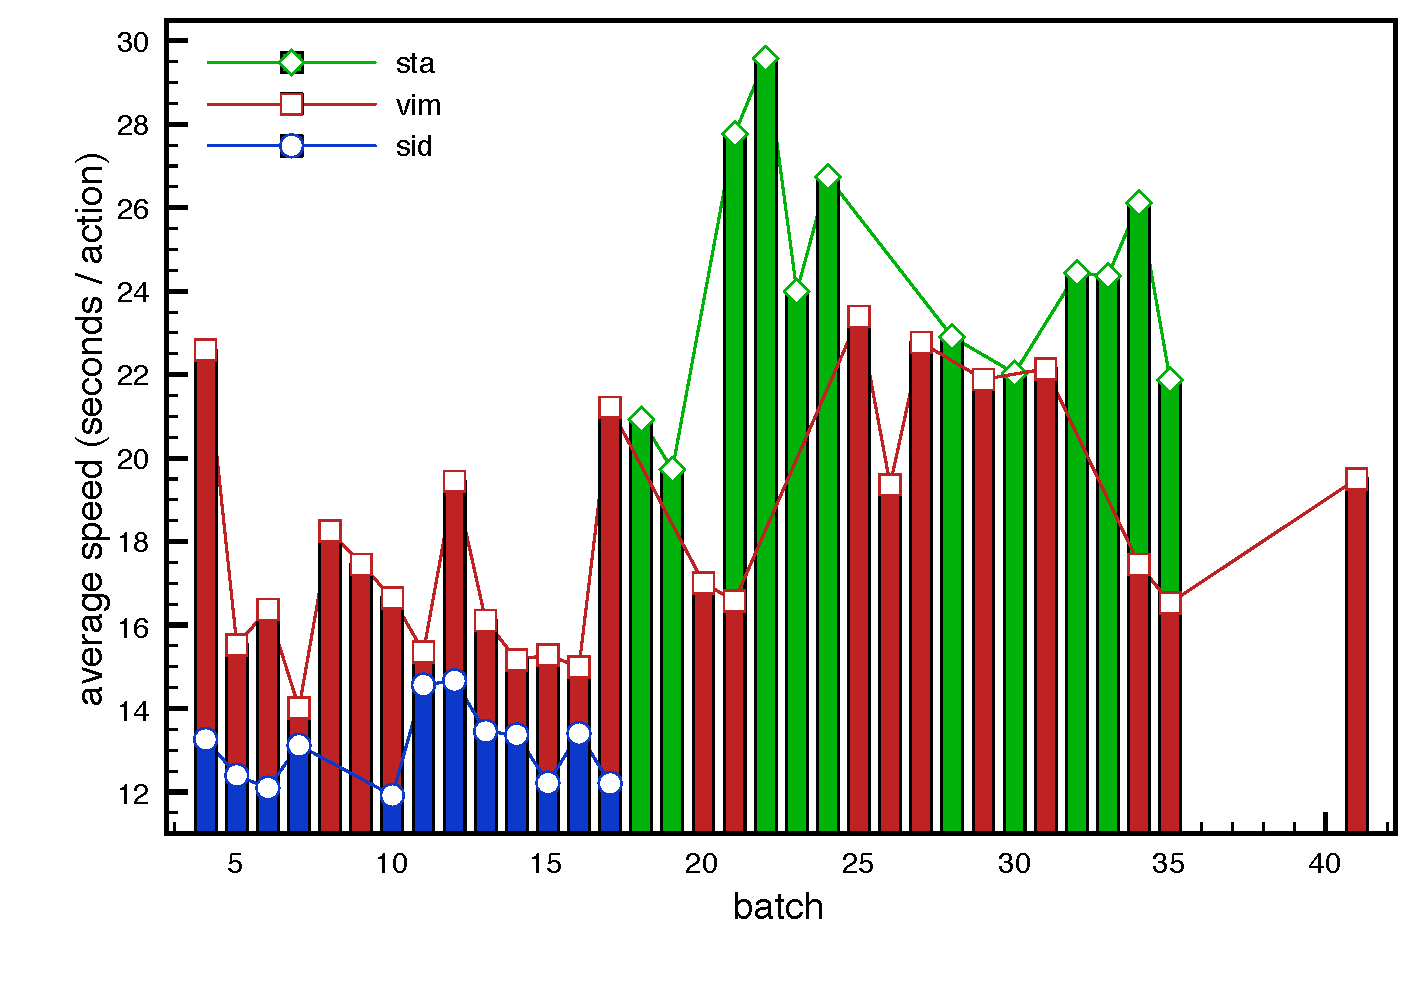
\includegraphics[width=\textwidth]{images/speed/speed-anot} 
   \caption{Average speed of each annotator for each batch that he/she annotated. We can see some inter- and -intra annotator variance in speed and some broad tendencies: annotators tend to have their own speed.}
   \label{fig:speed}
\end{figure}

\todo \xxx{problem toho, co vlastne vidime, jak nastavit pocitani, nas skript, zakladni udaje, grafy}

% !TEX root = ../disertace.tex
%!TEX encoding = UTF-8 Unicode

\chapter{\sdata}
\section{The design and the PML schema}
\sdata\ means s-layer PML files and the PML schema of these files. The idea behind \sdata\ design is to have a simple way to store additional ``sense'' annotations over any layer of PDT. The annotations are stored as a set of ``sense'' nodes. Each s-node contains a link to a sense repository (annotation lexicon) and a set of references to nodes (m-, a- or t-) that correspond to an instance of the sense. An \sf\ is thus basically a very simple flat list of \sn{}s. It does not contain any trees. A single \sf\ can only reference a single PDT file: either tectogrammatical, or analytical, or even morphological layer can be used, but references to different layers cannot be mixed in one s-file.

The design of \sdata\ is quite universal. S-files can be used to provide additional annotations over any PML files that contain nodes with IDs. The sense repository (annotation lexicon) can be any dictionary that provides IDs for the entries. The tools used in our annotations mostly expect PDT PML or the particular \sf{}s that we have used, but that is mostly for convenience. Should the need appear to adapt the workflow a different corpus represented by PML files and a different annotation lexicon, the changes required would be rather minor.

\section{Visualisation}
There are two basic ways to view st-nodes: in \seman\ or in \tred. Both of these need to use the ``t-a-m-w-'' PDT files to display the sentence and/or the tree for each sentence and then they read the \stf\ to add the information about \stn{}s. The \stn{}s are displayed as colour boxes or bubbles over the words in a sentence or nodes in a tree in \seman\ or \tred\ respectively.

\subsection{Visualisation using \seman}
The visualisation of annotated files in \seman\ has the advantage of showing whole text with all the \mwe{}s clearly marked in a single glance. Integration of the SemLex browser is also beneficial, because it allows fast and convenient lookup of annotated \mwe{}s in \seman. Details of \seman\ interface are described in \Sref{sec:seman}. 

There are, however, also some drawbacks of this ``full plain text of an article'' approach: 

\section{\tred\ extension}
\tred\ has a powerful mechanism that allows it to be extended for new tasks. We developed an extension \texttt{pdt-t-st} that allows to see MWEs as graphically marked groups of tectogrammatical nodes. 

 Main features of the extension:
 \begin{itemize}
\item
Merges the \stf{}s into \tf{}s and allows to display these enriched tectogrammatical trees.
\item
Types of annotated MWEs (i.e. types of NEs and \semlex\ entries) are distinguished with the same colours that were used in \seman\ during annotations. This allows not only for easily seeing NE types, but also easily spotting annotators' disagreement on them. 
\item
Allows to merge annotations of several annotators into one \tf. 
\item
Each annotator's MWEs have a unique raster. It is thus easy to spot annotators' partial or full disagreement not on types of MWEs, but also on their spans.
\end{itemize}

 There are two ways to merge the \sdata\ and \tdata: 
 \begin{enumerate}
\item
Merge on opening the \stf\ in \tred, and
\item
Static merge that produces the merged \verb=*.t.mwe.gz= file. 
\end{enumerate}
The dynamic merging is done using a newly developed feature of \tred\footnote{Developed by Petr Pajas} that allows to apply arbitrary perl transformations on the input data. Thus we open the \stf, use the mechanism of extensions to activate our extension by identifying the \stf\ as data the extension can process and call our transformation. The transformation requires a \tf\ annotated by this \sf\ to be present in the same directory. The \tf\ and \sf\ are parsed, and for each \stn\ we find a tectogrammatical tree that includes \tn{}s annotated (i.e. referenced) in this \stn. When we have a root of the correct t-tree, the \stn{}s are basically added into an attribute \texttt{mwes} of this t-root. The attribute is rather complex, because it contains lists of \stn{}s for all annotators that annotated any \stn{}s in this tree. Some small transformations of \stn{}s are needed, as well as creation of some new XML nodes, to represent the information from \sf{}s in the \tf{}s properly. For all the details inspect the code of \verb=$pdt_t_st/libs/SDataMerge.pm=.
%!TEX root = ../disertace.tex
%!TEX encoding = UTF-8 Unicode

\chapter{\seman}
\label{sec:seman}
The annotation tool \seman\ is written in Perl 5\footnote{\url{www.perl.org}; \url{dev.perl.org/perl5}} with Perl/Tk\footnote{\url{http://search.cpan.org/~srezic/Tk-804.029/}} GUI toolkit. The annotation tool depends on working installation of \tred, specifically its unix installation, because it uses \texttt{nTrEd} for efficient execution of \tred\ scripts in the background. \texttt{nTrEd} however, unlike \tred\ itself or \texttt{bTrEd}, does not work on Windows.% because it uses unix sockets.

% sem-ann screenshot 
\begin{figure}[htbp]
   \centering
   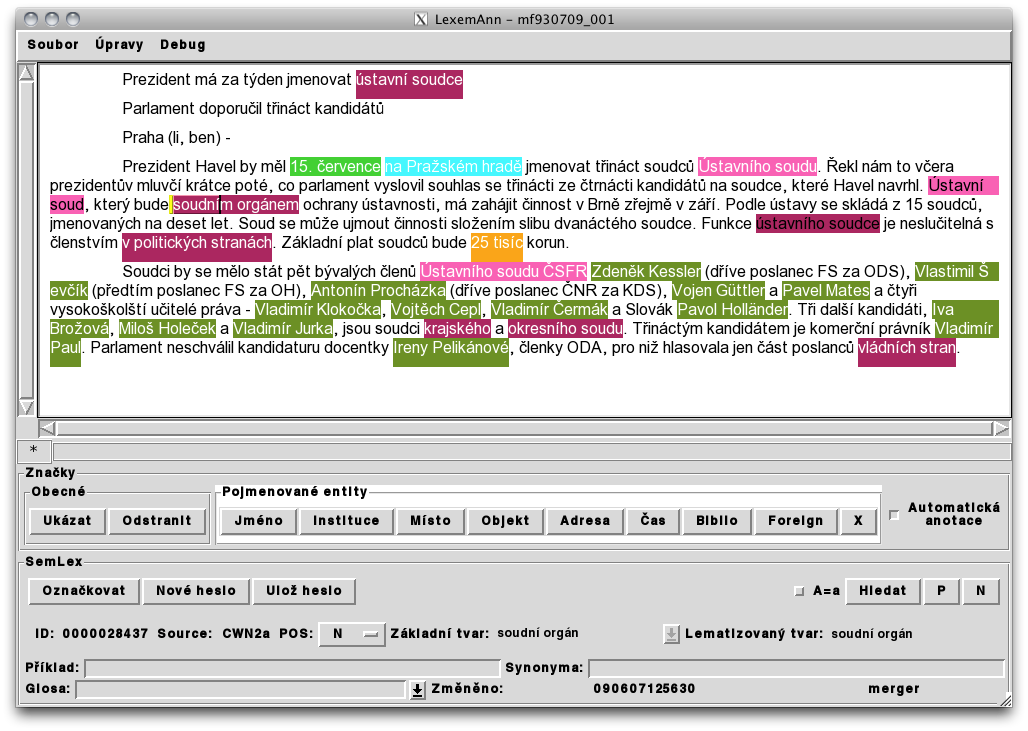
\includegraphics[width=.9\textwidth]{images/sem-ann2.png} 
   \caption{An annotated document in \seman. the yellow ``selection tag'' is barely visible on the word \pr{soudním}, because over a  different colour tag, selection has just a bezel. The \semlex\ entry that is displayed in the Semlex-part of the UI -- \pr{soudní orgán} -- is the one used to annotate the selected word. The black font colour in two tags distinguishes automatically pre-annotated MWEs.}
   \label{fig:seman-gui}
\end{figure}

\seman\ itself is composed of several main parts:
\begin{itemize}
  \item The main application file \code{sem-ann.pl} mostly implements the application frontend. It implements the GUI, loads an \sf, a \semlex,  and a log file for this \sf, if it had already been annotated. Then it takes care of all the interaction with the user and writes \sf, \semlex, and a log file.
  \item \ntred\ backend that is used to 
	\begin{itemize}
	  \item generate surface sentences from tectogrammatical trees in \tf{}s that are then displayed in the \seman\ GUI,
	  \item perform all the on-the fly pre-annotations (\Sref{sec:annot:pre})
	\end{itemize}
A \tred engine without a GUI with a few modifications aimed towards batch processing is called \btred. \ntred is essentially a modification of \btred that allows it to run as a daemon and process scripts over a network. We opted for \ntred, even though we ran it locally, because it can run as a daemon, thus eliminating a significant startup penalty of \btred. What we call ``\ntred\ backend'' is thus the running \ntred\ instance itself (that is started by the \seman\ during start-up, if there has not been a running instance detected), and the scripts used to generate the sentences that are displayed in \seman\ and to pre-annotate MWEs using their tectogrammatical tree structures.\footnote{these scripts were written entirely by E. Bejček~(\citeyear{bejcek:2010}).}
  \item The module \code{SemLex.pm} is used to read, save, query, and edit \semlex.
    \item The module \code{SemLex\textunderscore{}heslo.pm} implements the \semlex\ entry: its structure, attributes and accessors.
  \item There is also a suite of miscellaneous scripts mostly for validation of annotated data, comparing and merging multiple annotations, merging annotators' \semlex{}es, computing reliability of annotations, and other small tasks related to annotation and managing the annotated data and \semlex{}es.
\end{itemize}

%%%%%%%%%%%%%%%%%%
\section{User interface}
\label{sec:seman:gui}
The user interface (shown in \Fref{fig:seman-gui}) is divided three main parts: The text widget displaying the annotated text, a row of buttons to create annotations by NE tags, show info on annotations, or remove tags, and an editor of \semlex. 



%%%%%%
\subsection{Text widget}
\label{sec:text-widget}
The text, displayed for the annotator, is generated from the tectogrammatical trees (using also information from lower layers). That is, why for each document to be annotated, all the PDT files must be present ( t-, a-, m-, and w-layer). 

It is possible to generate the surface (plain text) sentence from a t-tree using the `built-in' function \verb=PML_T::GetSentenceString($root)=. Such a sentence is complete, correct, has correct spacing around punctuation, but it contains no relation to the t-layer anymore. And we want to keep this connection in order to be able to annotate the t-nodes, not just words \see{sec:annot}. Thus Eduard Bejček wrote the script \url{get_sent_t-layer.btred}, that creates a representation connecting words in a sentence with tectogrammatical IDs of the t-nodes from which these words are generated. This representation is actually input into the text widget and everything but the words is hidden from the annotators' view. \emph{The tecto-IDs are then what gets really annotated, \emph{using} the words.} The full representation can, however, be displayed using Debug menu commands. It is shown in \Fref{fig:seman:hidden} in comparison to the ``plain text'' as normally displayed (with no actual annotations to keep the view simple).

%% comparison of plain text and the same with hidden text -- screenshots%%
\begin{figure}[htbp]
   \centering
   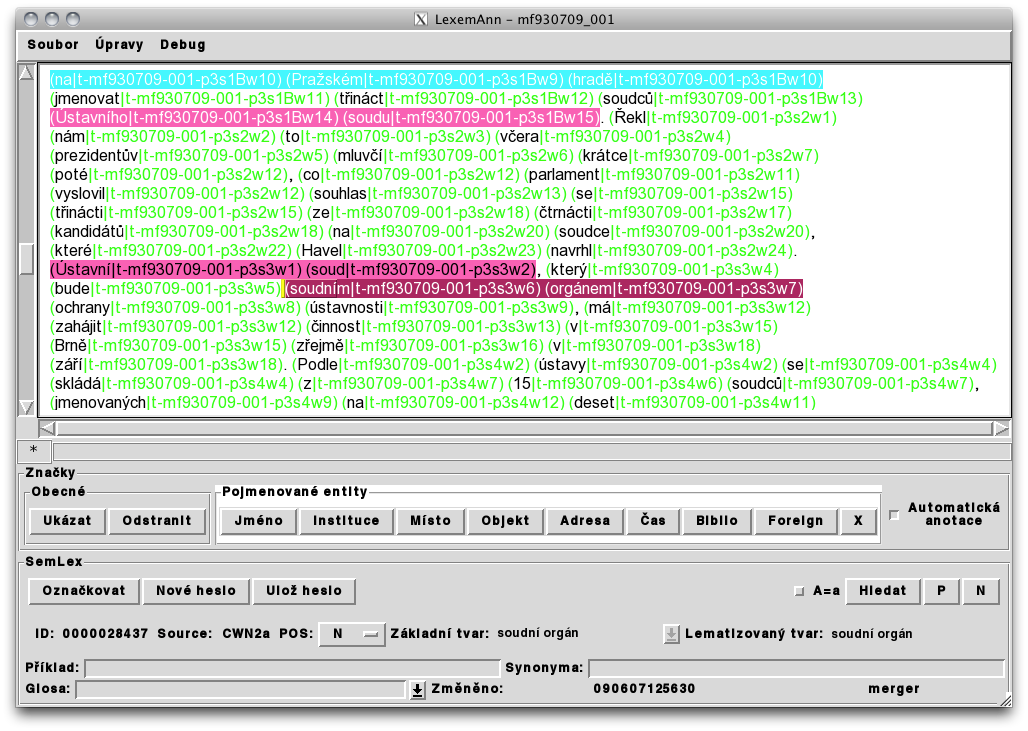
\includegraphics[width=.95\textwidth]{images/hidden-text2}
   \caption{Comparison of the plain text, as normally displayed, and the underlying representation that is used to relate the actions of annotators who mark words, to the references to tectogrammatical nodes that are actually saved in the annotation files.}
   \label{fig:seman:hidden}
\end{figure}



%%%%%%
\subsection{Annotation buttons}
The row of buttons below the text widget and the status bar is rather straightforward: 

The first group (from the left) contains two buttons that are connected to general commands used for all annotations (NEs and other \semlex\ entries alike). The first button shows a tag (i.e. the corresponding \semlex\ entry), on the word in focus (the word that is selected, or in which the cursor is placed). The second button removes the tag on the word in focus.

The second group of buttons simply creates NE tags over the selection. 

The last check button toggles the on-the-fly pre-annotation of other instances of the same MWE that annotator annotates, in the rest of the text (pre-annotation type~\ref{pre-on-annot}, see p.~\pageref{pre-on-annot}).



%%%%%%
\subsection{SemLex editor}
The \semlex\ editor and browser (see the lower part of \Fref{fig:seman-gui}) simply displays SemLex entries, allows to edit them, or to search SemLex by basic or lemmatised forms (see~\Fref{fig:semlex-search}), and browse the search results (using their basic forms). There is also a function to annotate the selected words (t-nodes) with the current SemLex entry. It is mapped simply to the return/enter key, once the focus moves from the SemLex part of the GUI to the text widget.

The attributes of an entry that are displayed include the basic and lemmatised form of an entry, its ID and source, example of usage, synonyms, if present, and a gloss. There is also a time stamp and a signature of the last modification. The attributes of a SemLex entry are explained in detail in \Sref{sec:semlex:entry}.

The search string is by default matched as a substring, and there is a check box to toggle case sensitivity. However when needed (and in case an annotator has the knowledge), full Perl regular expressions can be used. 
\begin{figure}[htbp]
   \centering
   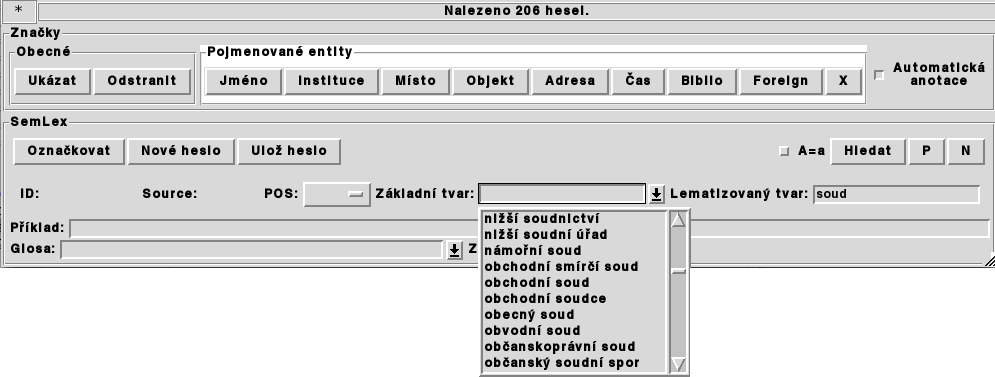
\includegraphics[width=\textwidth]{images/semlex-search}
   \caption{A result of a search in SemLex by a substring of the lemmatised form: 206 entries were found (see the status line at the top). Browsing the basic forms of the results.}
   \label{fig:semlex-search}
\end{figure}

%%%%%%
\subsection{General UI remarks}
Inspired by command mode of modal text editors and by some annotation regimes of \tred, we made all the annotation commands single-letter. That was made possible by making the text read-only. Since the letters are not used for input, they can be mapped to commands. All the command (and so the buttons) are named (in Czech) in such manner, that their first letter can be mapped to perform the command. Only the command for removing annotation is mapped to the capital letter (`O' for `odstranit') for safety reasons.


%%%%%%%%%%%%%%%%%%%
\section{Annotation logs}
\label{sec:logs}
An important, and as far as we know unique, feature of \seman\ is the design of annotation logs. As soon as an \sf is loaded in \seman, a \verb=*.st.log= file is created and every action taken henceforth, that modifies the \sf, is logged, together with a timestamp. 

Logs are saved in YAML format and timestamps are human readable on purpose. Thus it is easy to visually inspect the logs in case of problems with sf{}s, e.g. data corruption. It was helpful on several occasions. However the main point of logs is different.

Logs are a source of valuable information that can provide an insight into what is actually going on during annotation. Analysis of logs together with s-files can help estimate the real cost of annotations, which we have done during annotations to some extent, by estimating speed of annotations \see{sec:time-analysis}. 
But the analysis can go further and, to formulate the problem in economic terms, try to examine in general what factors influence the price of a (correct) tag. What is the relation of speed, length of work intervals, time of day, order of processing of the file, and other factors? We give only a very brief glimpse of one of the factors -- speed of annotations in \Sref{sec:time-analysis}, but in our opinion thorough statistical analysis of log files is an important source of information also for future annotation projects. \xx{Presunout odstavec do casove analyzy ve Future Work?}

The log files are however useful also directly to annotators during their daily work, because they provide information necessary for persistent undo and redo. Even when the file has been partially annotated long time ago, an annotator can review the last steps taken and continue with more information.

%!TEX root = ../disertace.tex
%!TEX encoding = UTF-8 Unicode

\chapter{SemLex}
\label{sec:semlex}

\section{Building SemLex – based on the JLRE article}
\label{sec:semlex:build}
Each entry we add into SemLex is considered to be a monosemic MWE. 
We have also added nine special entries to identify NE types, so we do not need to add all the expressions themselves.

\section{Named entities}
\label{sec:semlex:ne}
\emph{Named entities} are a concept originating in information retrieval (??, quote). This concept is well rooted in NLP but it does not exist in classical lexicology and its defining criteria do not correspond with a definition of a lexical unit, lexeme, or any other lexicological or lexicographic concept of our knowledge.

We used the NE classification by \citet{sevcikova:2007} as a starting point. However the definition of what the named entities are is problematic:
\begin{quote}
\textczech{\em „Pojmenované entity jsou jednotlivá slova nebo slovní spojení, která v textu vystupují jako
pojmenování osob, míst, firem apod. Cílem anotace je označení všech pojmenovaných entit v 
předloženém lineárním textu. Současná anotace bude zaměřena na identifikaci
především těch pojmenovaných entit, které jsou zapsány s velkým počátečním písmenem.“}
\end{quote}
The definition basically says that named entities are single- or multi-word units that are used to name persons, locations, firms, etc. I.e. named entities are the expressions used to name entities. It is actually hard to call this a definition at all.

It is nevertheless not easy to define named entities properly. Other authors do not fare much better: \xxx{definice sem!}

We believe we can provide at least some additional constraints to the definition above: To be considered a named entity an expression must share at least some \xxx{(or all ??)} \emph{features of idioms}: it cannot be an exploitation \citep[see][]{hanks:norms}, i.e. it must fulfill some criteria of stability. \xxx{Any more??}

Our types of entities are:
\begin{compactenum}
\item ``a~name of a person or an animal'', 
\item``institution'', 
\item``location'', 
\item``other object'' (used for names of books, units of measurement, biological names of plants and animals), 
\item``address'', 
\item``time'', 
\item``bibliographic entry'', 
\item``foreign expression'' and 
\item``other entity''
\end{compactenum}

Compared to the original, the classification is altered because we do not use embedded entities. In the original, \citeauthor{sevcikova:2007} use a bracketing approach, in which entities of all types are further structured into smaller parts. We also altered some rules for classifying particular types of entities as follows:
\begin{itemize}
\item  We do not distinguish \emph{names of animals} as a distinct type. Animal names are considered the same type as the names of persons.
\item We also merge the \emph{names of media} (newspapers, TV stations, \ldots) with names of companies. The reasons are mainly: a) it seems arbitrary to distinguish specifically names of media. b) It is also often hard to distinguish whether a name is a name of media or a company that owns or runs the media. At the same time there is usually little reason to try to make this distinction.
\item \emph{Numbers with non-quantifying meaning} are merged with addresses. Since the subtypes defined for this type are \code{zip code}, \code{street number} and \code{phone/fax number}, this merge is quite natural, especially since these occur mostly as parts of addresses and we do not annotate any embedded entities.
\end{itemize}

Some frequent names of persons, institutions or other objects (e.g.~film titles) are being added into SemLex during annotation (while keeping the information about their NE type), because this allows for their following occurrences to be pre-annotated automatically (see Section~\ref{sec:annot:pre}). For others, such as common addresses or bibliographic entries, it makes but little sense, because they most probably will not reappear during the annotation. 

\section{Lexemes from other dictionaries}
\label{sec:semlex:dicts}
The base of \semlex\ has been composed of MWEs extracted from Czech WordNet \citep{smrz:03}, Eurovoc \citep{eurovoc:07} and Dictionary of Czech Phraseology and Idiomatics \citep{cermak:1988}.%
For the explanation of our use of the SČFI subset see point \ref{pre-hnatkova} in Section~\ref{sec:annot:pre} below. 
\xxx{update: Currently there are 32196 MWEs in SemLex (po sliti a dokonceni davky 42).}

\xxx{In the current ``compiled'' SemLex there are many collocations that can hardly be considered MWEs. However, these frequently occurring collocations are pragmatically quite useful and it may be good to identify them, too.\footnote{We would like to mark these entries in SemLex at some point, so that we know these in fact are not MWEs and we do not attempt to create a single t-node for them when they are annotated.} The most important thing is to ensure that they are annotated consistently. They can be useful for machine translation, because, e.g., for those collocations that were extracted from Czech WordNet, there are at our disposal their translations into English (CWN). For the collocations that come from Eurovoc we even have translations into all the official languages of the European Union.}

The entries added by annotators must have defined their ``sense''. Annotators define it informally (as well as possible) and we extract an example of usage and the basic form from the annotation automatically. The ``sense'' information will be revised by a lexicographer, based on annotated occurrences.

\subsubsection{Eurovoc}
\label{sec:semlex:eurovoc}

\subsubsection{CWN2a}
\label{sec:semlex:cwn}

\subsubsection{SČFI}
\label{sec:semlex:scfi}


\section{Structure of \semlex}

From the technical point of view, \semlex\ is a simple list of entries. It is stored in YAML format, which makes it easily readable in its source form using any Unicode-aware text editor. Since YAML is a data serialization format and not a markup language, it can also store information needed to represent data as objects in the Perl OO model. 

In addition to the \semlex\ itself we also build an index of basic forms on some special occasions. It is not needed during annotation, so we do not create the index normally but it can be called by passing a second parameter\footnote{The parameter is evaluated as a BOOL type.} to the function \verb=SemLex::load_yaml()=. 

\subsection{\semlex\ entry}
\label{sec:semlex:entry}
An entry is composed of several user-editable attributes, and some read-only and machine-generated metadata:\footnote{By ``user-editable'' we mean editable in \seman. Everything is of course editable in the YAML source format using a text editor, but that is not what a typical user that we have in mind does.} 
\begin{verbatim}
  - !!perl/hash:SemLex_heslo 
    BASIC_FORM: vysoké kruhy
    CREATED: 070115163056
    EXAMPLE: ''
    GLOSS: ''
    ID: 0000017495
    LEMMATIZED: vysoký kruh
    MODIFIED: 090607124212
    MODIFIER: merger
    MORPHO_TAGS: AAIP2----3A---- NNIP2-----A----
    ORIGID: ''
    POS: ''
    SOURCE: SCFI
    SYNONYMS: []
    TREE_STRUCT: "--- []\n\n"
\end{verbatim}

\begin{description} % atributes of a SemLex entry
\item [- !!perl/hash:SemLex\textunderscore{}heslo] -- The first line of a \semlex\ entry provides a lot of information. We describe its parts from the left to the right:
    \begin{description}
    \item [- ]The hyphen at the beginning of the line, together with indentation of the lines that follow, indicates that this is an array element in YAML. Remember that we said that SemLex is a simple list of its entries. Thus we chose to implement is with an array, as it is both sufficient and very efficient.
    \item [!!perl] This string says that the array element actually represents a serialisation of a Perl object.
    \item [/hash] The object is implemented as a hash.
    \item [:Semlex\textunderscore{}heslo] The object belongs to the class Semlex\textunderscore{}heslo.
  \end{description}
\item [BASIC\textunderscore{}FORM] -- The basic form of a lexeme. We could call it a ``lemma'' of a lexeme, but we do not find it suitable for several reasons: 
  \begin{itemize}
    \item In many languages including Czech it often contains word forms in other than the basic form for the given word on its own. I.e. ``vysoké učení'' contains a feminine suffix of the adjective ``vysoký'' (high) because of the required agreement in gender with the noun, whereas the traditional lemma of adjectives in Czech is in the masculine form.
    \item  It could be confused with the attribute ``lemmatized'' that means something completely different.
  \end{itemize}

\item [EXAMPLE] -- An example sentence or collocation that illustrates the prevalent use of the MWE

\item [GLOSS] -- Primarily used for an explanation of the MWE, much like in traditional dictionaries.

Secondary use of this attribute is for additional notes or processing instructions. Annotators put specially formated notes into this field to mark that the entry has some special property that we do not have an attribute for, that the entry should be removed, or they could indicate that they have just some other note for the entry. This secondary use of GLOSS and  the type of note was marked by special format of the beginning of the note:
    \begin{description}
    \item [\code{***(<type>)}] -- The entry is a NE that the user wants to add into \semlex. The usual reason is that the NE is common in the annotated text. When it is added into \semlex, it can be pre-annotated automatically more efficiently (see \Sref{sec:annot:pre} for details). \code{<type>} means that at this place there is a name of one of the types of NEs as described in \Sref{sec:semlex:ne}.\footnote{The notes actually use Czech names of these types.} 
    \item [\code{***derived from: <ID>}] -- The entry is derived from another entry that already exists in \semlex. \xxx{popsat, rozsirit. Nemela by to byt subsekce a odkaz?}
        \item [\code{***remove}] -- The entry is not a MWE, thus its instances should not be annotated and the entry should be removed from \semlex.
        \item [\code{***<anything else>}] -- Other notes. The entry must be inspected and something (other than removing it) must be done.
  \end{description}
  
\item [LEMMATIZED] -- ``Lemmatised \code{BASIC\textunderscore{}FORM}'', i.e. take the basic form of an entry and substitute each form with its morphological lemma. This attribute is used for pre-annotation of entries that have not been annotated yet, so their tree structure has yet to be identified. For more details see Section~\ref{sec:annot:pre}  on page \pageref{sec:annot:pre}.\label{lem}

\item [MODIFIER] -- For newly created entries, this attribute is empty regardless whether they were created by modifying entries from other dictionaries during original creation of SemLex, or whether they were created by annotators during annotation. Is is used to mark that the entry was modified after its creation and who last modified the entry. See \ref{lem}

\item [MORPHO\textunderscore{}TAGS] -- Morphological tags corresponding to the \code{BASIC\textunderscore{}FORM}. The tags were acquired automatically by running the morphological tagger of Jan Hajič (\citeyear{hajic:2004}). This is a suplementary information that has not been used during later stages of annotation. It was implemented for pre-annotation using only morphological layer or alternativelly only plain text and morphological tagger. After some initial testing we have not used this pre-annotation, so it does not appear in \Sref{sec:annot:pre} and it is not implemented in current \seman\ workflow. 

The morphological tags could however still prove useful if \semlex\ should be used for annotatiuon of resources without tectogrammatical layer. Then it could be useful to employ this type of simpler pre-annotation.

\item [ORIGID] -- If the entry comes from some other existing dictionary, this is the original ID of the entry in that source dictionary (identified by the attribute \code{SOURCE}).

\item [POS] -- The part of speech of the entry as a unit. Usually it corresponds to the part of speech of the syntactic head of the entry in terms of the underlying tectogrammatic tree structure, but there are some exceptions:
% POSes:
  \begin{description}
    \item [N] -- noun; 
    \item [A] -- adjective; \pr{trvale udržitelný, ekonomicky aktivní, do očí bijící}
    \item [V] -- verb; \pr{působit jako blesk z čistého nebe (\xxx{really???}), zaujmout stanovisko, mít dohled, spadl (komu) kámen ze srdce}
    \item [D] -- adverb; e.g. \pr{mezi čtyřma očima, na lavičce\footnote{Trenér Borovička se zatím nerozhodl, zda král střelců Siegl začne v základní sestavě, nebo zase jen na lavičce.}}, or \pr{o dům dál}
    \item [I] -- interjection;
    \item [F] -- foreign; often Latin, Greek, but also other idioms that are already ``native'' to the Czech language enough to include them in a dictionary instead of annotating them just as a foreign entity, e.g.~\pr{hip hop, a la, de iure}.
    \item [N/A] -- not applicable; used for proverbs, sayings, other idioms forming whole sentences, or idioms with unclear part of speech, e.g. \pr{stručně řečeno; stal se kozel zahradníkem, Tady je dobrá rada drahá.}
  \end{description} % end POSes

The entries in the original \scfi\ do not carry the information on the part of speech, so we were not able to fill the attribute in the beginning. Thus the entries from \scfi\ have the POS information only in case they were manually edited. In that case the POS is always added, because the \seman\ interface does not allow the edited entry to be saved without indicating the part of speech.\footnote{For details of the \seman\ user interface to \semlex\ see \Sref{sec:seman:gui}.} % end of item [POS]

\item [SOURCE] -- Where did the entry come from. Possible values are {\tt CWN2a}, {\tt Eurovoc}, {\tt SCFI}, or {\tt <annotator>}. {\tt <annotator>} means that the entry was created during annotations and stands for an identifier of the annotator who created it. An annotator found a MWE, searched the \semlex\ for the expression, and decided a new entry is needed. When the entry is created, the annotator's identifier is written as the SOURCE. This attribute is used to trace the origin of entries during analysis of annotations and when merging individual annotators' SemLexes. 

When the entry is a result of merging several entries from different sources (either different source dictionaries or several annotators created the same entry), the value is a concatenation of the sources. In case that automatic merge was not possible \code{SOURCE} 

\item [SYNONYMS] -- A list of synonyms (implemented as an array). In case of Entries from WordNet, the synsets were split to individual entries, but the relation between them was kept via the ORIGID attribute and the basic forms of the synonymous MWEs were copied into this attribute as the synonyms of the MWE. This attribute helps annotators to understand an entry's meaning, especially since most synsets in the WordNet did not have any glosses or examples. See \Sref{sec:semlex:cwn} for more information on entries derived from WordNet. Occasionally annotators added synonyms manually, if they just happened to think about them when using an entry. It was however by no means systematic work and it was not one of the goals of annotation.

\item [TREE\textunderscore{}STRUCT] -- The tree structure of an entry. This is a simplified tectogrammatic representation of the entry and is a key to the most advanced pre-annotation that we employ: identification of future occurrences of the same tree structure in the text. This pre-annotation requires \ntred. See discussion of various types of pre-annotation in \Sref{sec:annot:pre}.

\end{description} % end - attributes of a SemLex entry


%%%%%%%%%
\section{Zajímavá hesla -- provizorni}
Some entries seem at the first look just wrong. A class of automobiles is a perfectly compositional collocation with clear syntactic structure, isn't it? However ``automobil nižší střední třídy'' is a different matter.
\begin{verbatim}
 - !!perl/hash:SemLex_heslo 
    BASIC_FORM: třída automobilů
    CREATED: 070926062821
    EXAMPLE: ~
    GLOSS: ~
    ID: 0000003520
    LEMMATIZED: třída automobil
    MODIFIED: 070926062833
    MODIFIER: sidak
    MORPHO_TAGS: ~
    ORIGID: ~
    POS: 'N'
    SOURCE: sidak
    SYNONYMS: []
    TREE_STRUCT: ''
\end{verbatim}

Creative use -- exploitation (Hanks). Very common in journalism. PDT is composed of daily news, so expolitations of this kind are quite common in our data too.
\begin{verbatim}
  - !!perl/hash:SemLex_heslo 
    BASIC_FORM: mezi osmi očima
    CREATED: 100622025530
    EXAMPLE: ~
    GLOSS: "***derived from 0000032132 (mezi čtyřma očima)"
    ID: 0000032133
    LEMMATIZED: mezi osm oko
    MODIFIED: ~
    MODIFIER: bejcek
    MORPHO_TAGS: ''
    ORIGID: ~
    POS: 'D'
    SOURCE: vimmrova
    SYNONYMS: []
    TREE_STRUCT: ''
\end{verbatim}

\subsection{Partial freedom in an idiom}
\pr{(rozčeřit | rozhýbat) stojaté vody}. Here it is (based on our data and knowleadge) only these two alternatives on this one position. However some idioms show much richer variation and the relations between the alternates are very complex. See \xxx{doplnit.} Due to the complex nature of these alternations we have kept the variants separate. Neither we nor the annotators are trained lexicographers to decide the cases. It would also require completely different setup, searching larger corpora, etc. The efficient approach during annotations was to create separate entries and link them via a special form of gloss, as below.  Thus we do not loose any information and leave it to the lexicographers to come up with a good description of the complex relations of these variants.
\begin{verbatim}
  - !!perl/hash:SemLex_heslo 
    BASIC_FORM: rozčeřit stojaté vody
    CREATED: 100622030630
    EXAMPLE: ~
    GLOSS: "souvisí s 0000029189 (rozhýbat st.v.)"
    ID: 0000032134
    LEMMATIZED: rozčeřit stojatý voda
    MODIFIED: ~
    MODIFIER: bejcek
    MORPHO_TAGS: ''
    ORIGID: ~
    POS: 'V'
    SOURCE: vimmrova
    SYNONYMS: []
    TREE_STRUCT: ''
\end{verbatim}

\pr{sloužit mši} je idiomatický rámec i ve Vallexu. Takovych je v nasich datech urcite mnohem vic -- \xxx{relation of our data to Vallex and PDTVallex}
\medskip

These should probably have been two entries -- for two POS'. \xxx{Jak je zpracované heslo 'postižený' v PDTVallexu?}
\begin{verbatim}
  - !!perl/hash:SemLex_heslo
    BASIC_FORM: zdravotně postižený
    CREATED: 080408072653
    EXAMPLE: ~
    GLOSS: subst. i adj.
    ID: 0000031992
    LEMMATIZED: zdravotně postižený
    MODIFIED: 100502113206
    MODIFIER: sidak_vimmrova_sidaklexicographer_vimmrova_sidaklexicographer
    MORPHO_TAGS: ''
    ORIGID: ''
    POS: N i A
    SOURCE: sidak_vimmrova
    SYNONYMS: ~
    TREE_STRUCT: ''  
    \end{verbatim}

% !TEX root = ../disertace.tex
%!TEX encoding = UTF-8 Unicode

\chapter{Conclusions and Future work}
\label{sec:conclusion}

\section{Conclusions}

Several years ago, we were thinking about the best way to begin working on improving the state of t-lemmas: to push them a bit forward, from the legacy of surface layer they still carry, towards deeper representation of lexical meaning. Our conclusion was, partly due to our previous experience with annotation using Czech WordNet as the annotation lexicon \citep{holub:2003,bejcek:2006}, was to start by identifying multiword expressions.

We came forward with two hypotheses based on the properties of dependency syntax and specifically of the tectogrammatical description: 1) That each MWE should form a single contiguous dependency structure, and 2) That all instances of a MWE should share the same dependency structure.

After examining a possibility of annotating t-trees directly we came with an idea of an annotation tool that presents a continuous plain text, but links the plain text to the underlying tectogrammatical structure, from which it is generated. 

We proceeded to implement the annotation tool. As an integral part of the tool, we created a system of several types of pre-annotation of data. The most effective pre-annotation is based on the assumptions about tree structures of MWEs. We also devised a simple and efficient way for storing the annotation in a (relatively) human readable and still PML-compliant form by introducing \emph{s-data}. As an important part of the annotation environment, we implemented detailed logs of the annotation that helped us to (at least to some extent) estimate the speed and price of annotation.

We also created a TrEd extension in order to be able to visualise and search s-data together with t-data in TrEd. The extension also provides means to create enriched t-layer that includes MWE annotation. This data can then be used for instance on a PML-TQ server without further dependency on the original s-data.

During our annotation two annotators at a time have annotated multiword expressions and named entities in the whole PDT 2.0 (t-layer). One of the annotators, who was with us for the whole duration of the project, actually annotated about half of the PDT herself.

One of the important result of the annotations is our annotation lexicon \emph{SemLex}: It consists of all the MWEs identified during annotations. All SemLex entries contain tectogrammatical tree structures 

In Section~\ref{sec:annot:pre} we show that the richer and the more consistent the tectogrammatical annotation, the better the possibilities for automatic pre-annotation that minimises human errors. In the analysis of inter-annotator agreement in \Sref{agreement} we show that a weighted measure that accounts for partial agreement as well as estimation of maximal agreement is needed. We present such a measure, deriving it from Cohen's weighted kappa.

The resulting $\kappa_w^U$ has actually been gradually improving (cf. \citealp{biblio:BeStAnnotationMultiword2008}) as we were cleaning up the annotation lexicon, and employing more pre-annotation.

%The methodology of MWE annotation we developed enables precise pre-annotation by automatically extracted tectogrammatical tree structures. We have shown that this pre-annotation should improve annotation speed and should improve also agreement.\footnote{However, we do not present proper statistical tests, so we do not claim, that it does improve the speed and consistency. Only that there are good reasons to believe so.} 

We have shown that the hypotheses about tree structures of MWEs hold, provided the tectogrammatical layer is correctly annotated.\footnote{The only exception (there must always be one, after all) is in the coordinating conjunctions: since our MWE tree structures are built using the ``effective parent'' relation, the coordinating conjunctions are left apart, as they are not the effective parents of their (non-effective) children nodes.} In this respect, our data, especially the places, where different t-structures were (on purpose!) annotated with the same MWE from SemLex, also provide valuable information for both correcting errors and implementing new features in future versions of PDT. 

The annotation tool \code{sem-ann} is freely available under a permissive licence. The annotated data and the annotation lexicon SemLex are also available and will be also published by the Linguistic data consortium. The TrEd extension is available to any TrEd user in the standard extensions repository and is available under the same permissive licence as \code{sem-ann}. For details on availability of tools, data, and licence, see \url{http://ufal.mff.cuni.cz/lexemann/mwe/}.

We believe, however, that we still didn't manage to to properly process all the information that we have acquired during annotation and interesting work still remains to be done.
%
%\section{rozpracovat}
%\xx{Co jsme udelali:} hypoteza o tekto stromech MWE, anotacni nastroj, datovy format pro data, vyuziti hypotezy v predanotaci, \semlex, jeho datova representace, t-stromecky v semlexu, extension -- zobrazeni anotaci a vyhledavani v nich; prvni data, o kterych vime, kde muze i uzivatel hledat shodu a neshodu, apod. (umozneno skvelymi nastroji jinych: PML, tred, pml-tq). Hypoteza potvrzena? Mimochodem anotaci nalezeny chyby v PDT, nektere systematickeho razeni (chybejici uzly v koordinacich?), a take se ukazalo, ze nas blokovaly nedokoncenosti t-lemmat (deminutiva, prechylovani).

\xx{Zhodnotit vysledky toho, ze nekdy se vyplati anotovat rucne}, a nekdy ne: pripad jmen osob. Zjevne jsme udelali chybu, ze jsme to neanalyzovali takto (viz data od PaSi - EB) drive a nepredanotovali zbytek automaticky podle PDT. Ovsem, nasli by pak anotatori to, co nasli, kdyz by si zvykli na velmi vysokou uspesnost predanotace?

\xx{Pravdepodobnostni pristup k idiomaticnosti} -- mira, nikoliv kategorialni velicina s hodnotami nic, frazem, idiom, ..., ale zaroven mame miru pro mereni vazene shody. 

\section{Future work}
% -- Further analysis of annotation logs
\label{sec:conc:logs}
Considering the price of annotation, it is interesting, how much the annotation process itself stays out of focus of the researchers who create annotated data. Reading the papers and listening to presentations on NLP conferences and the various annotation workshops, one cannot help but see this approach: The data is very interesting, so let us just create it somehow. Almost never is there any published information on the annotation process, factors that influence quality of data, or the price of the results. 

Logs are a  very good source of this valuable information. They can provide an insight into what is actually going on during annotation. Thorough statistical analysis of the logs can provide unbiased information that is hard to get any other way. Better analysis of logs together with s-files can perhaps improve estimation of the real cost of annotation. We have done this during annotation to some extent \see{sec:time-analysis}, but our method is not particularly sophisticated and we just more or less guessed the fluency constant for the annotation intervals.
 
As a small sample of what can be done with the data, we present some further information on the time aspect of annotation work. We decided to have a look at the distribution of times between two consecutive annotation actions\footnote{A helpful suggestion of Zděněk Žabokrtský.}. We hoped that it can give us more information for properly handling the fluency of annotation intervals discussed in \Sref{sec:time-analysis}. 

We leave it to real statisticians to examine the data more carefully. What is however quite striking in the plots in \Fref{fig:hist} and \Fref{fig:hist-detail}, is the similarity of the histograms. Even though they are not normalised to disregard the different amount of data annotated by each person, the distributions point to a remarkable similarity in behaviour of all three annotators. Compare for instance the distribution for the times up to five seconds. We do not have any explanation or even hypotheses for the uniform raise at 1 second\footnote{histograms actually indicate a lower bound of an interval. 2 seconds thus means $\langle1, 2)$, etc.}, drop at 2, raise at three, etc. It seems to be an interesting point to examine, however.

\begin{figure}[htbp]
   \centering
   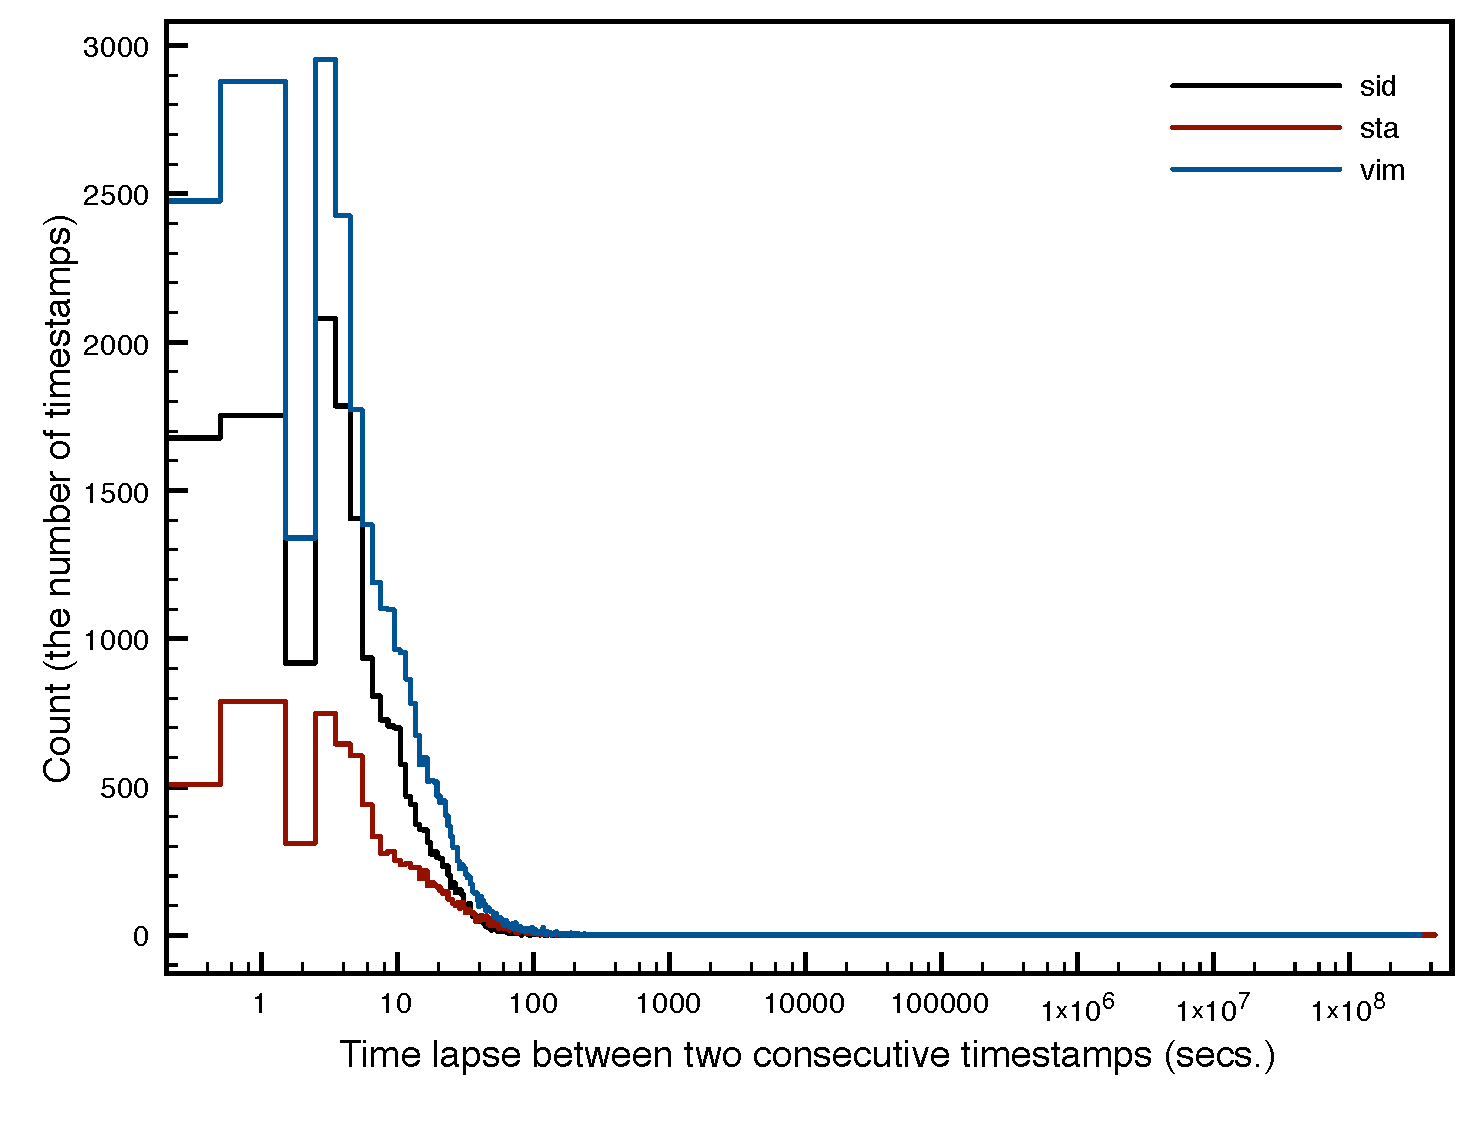
\includegraphics[width=.8\textwidth]{images/speed/histograms} 
   \caption{A histogram showing how many times ($y$) did an annotator place the next tag exactly $x$ seconds after the previous one.} 
   \label{fig:hist}
\end{figure}

\begin{figure}[htbp]
   \centering
   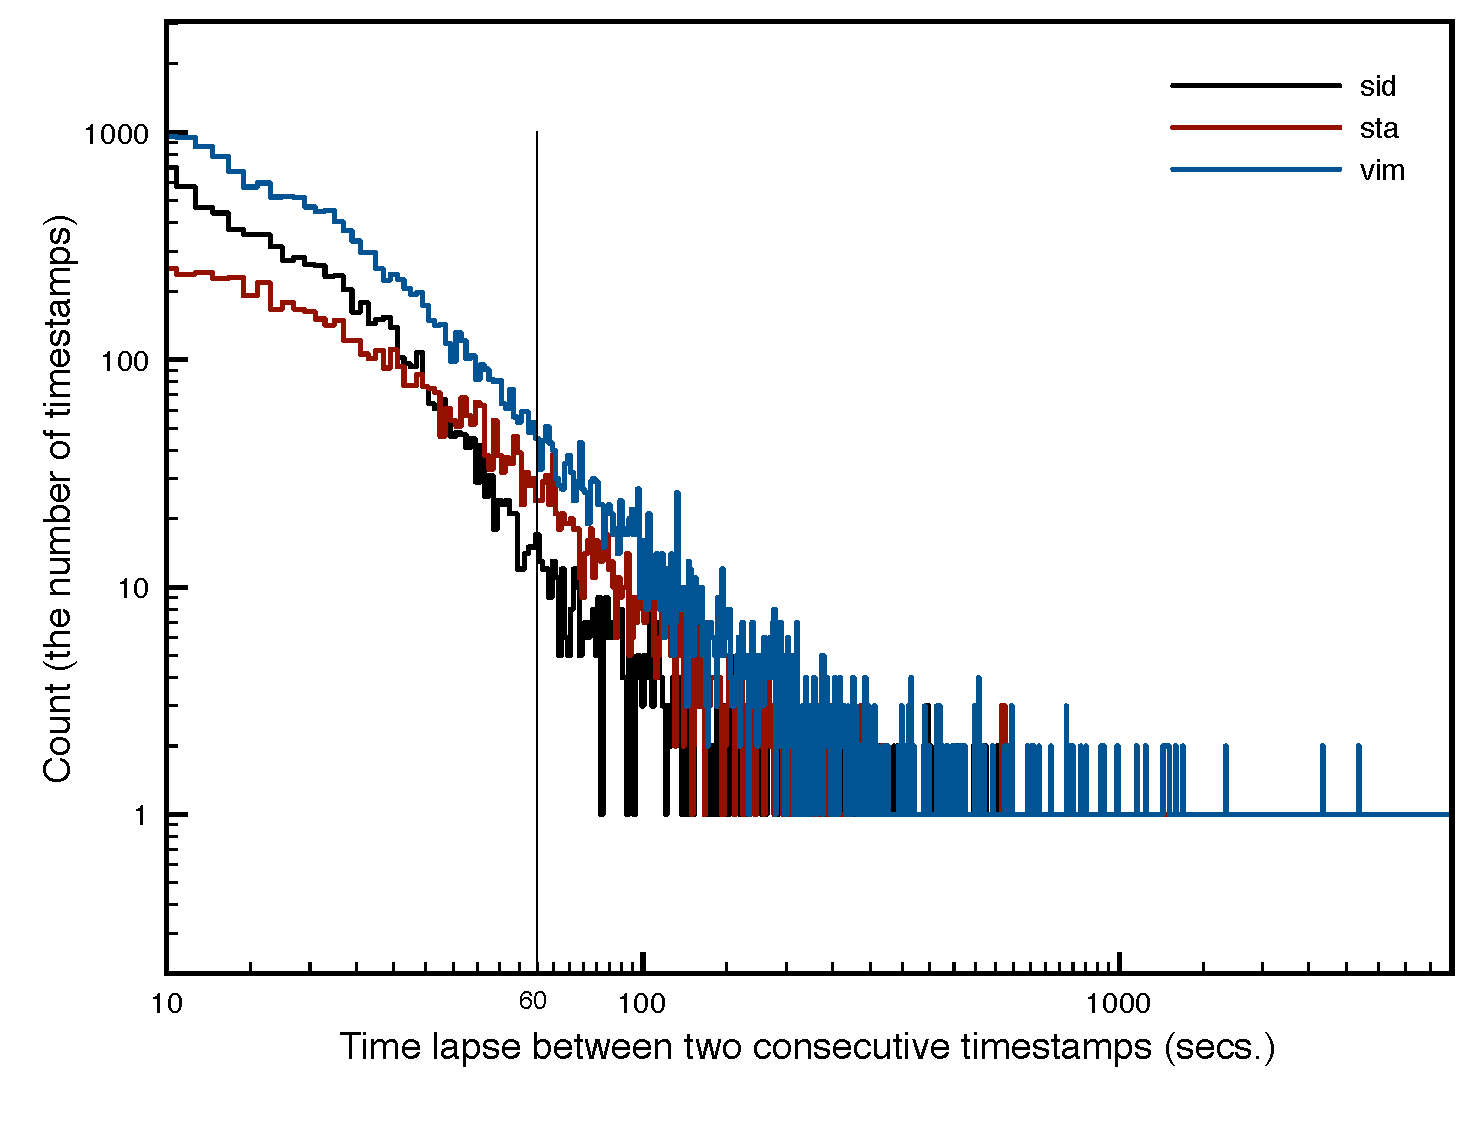
\includegraphics[width=.8\textwidth]{images/speed/histograms-detail} 
   \caption{Detail of the histogram in \Fref{fig:hist} in an interval where we have placed our \emph{fluency} value for the preliminary experiment with clustering of work into annotation intervals ($f=300$, see \Sref{sec:time-analysis} and \Fref{fig:speed}).}
\label{fig:hist-detail}
\end{figure}


But the analysis can go further and, to formulate the problem in economic terms, try to examine in general what factors influence the price of a (correct) tag. What is the relation of speed, length of work intervals, time of day, order of processing of the file, and other factors? We give only a very brief glimpse of one of the factors -- speed of annotation, but in our opinion thorough statistical analysis of log files is an important source of information also for future annotation projects. It may be possible to maximise the efficiency of annotation by experimentally identifying the positive and negative factors. Some of the factors can be quite universal, such as worse concentration after $n$ hours of work, but some may be quite individual (e.g. working in the morning, or on Saturdays\ldots). If some positive and negative factors influencing annotation can indeed be identified, annotation guidelines, both for the project and for the individual annotator can be appropriately modified to maximise the positive and avoid the negative factors.

It is of course possible that in the end no such factors can actually be estimated reliably, at least from our data. But currently we are in a position to seriously examine the possibility and to find out. That is more than has been done until now in any annotation project that we know of. From the little that we can see from our limited experiments, there is already some interesting data that requires interpretation.



\bibliographystyle{plainnat}
\bibliography{Bibliografie}
\end{document}